\documentclass[11pt]{article}

\usepackage[margin=1in]{geometry}
\usepackage{amsmath,amssymb,amsthm,mathtools}
\numberwithin{equation}{section}
\usepackage{booktabs,tabularx,array}
\usepackage{graphicx}
\usepackage{caption}
\usepackage{float}
\usepackage{enumitem}
\usepackage{xcolor}
\usepackage{tikz}
\usetikzlibrary{positioning,arrows.meta,shapes.geometric,decorations.pathreplacing}
\definecolor{mechnavy}{RGB}{25,62,96}
\definecolor{mechteal}{RGB}{27,125,129}
\definecolor{mechrust}{RGB}{157,77,50}
\usepackage[round]{natbib}
\usepackage[expansion=false]{microtype}
\usepackage{setspace}
\onehalfspacing
\usepackage{titlesec}

% Compact run-in headings within each numbered subsection.
\titleformat{\subsubsection}[runin]
  {\normalfont\normalsize\bfseries}{\thesubsubsection}{0.6em}{}
\titlespacing*{\subsubsection}{0pt}{0.6\baselineskip}{0.6em}
\usepackage{hyperref}

\graphicspath{{../figures/}{figures/}}
\newcommand{\NT}{../../output/model/experiments/transitions_2023/notag_7p9/output/model/experiments/transitions_2023/7p9167_v6}
\newcommand{\EXP}{../../output/model/experiments/transitions_2023/7p9167_v6}
\newcommand{\MECH}{../../output/model/production_runs/2026-10-12_comparison_7p917}
\newcommand{\TRANS}{../../output/model/production_runs/2026-10-11_transition_7p917/fitted_path_figure}
\hypersetup{
  colorlinks=true,
  linkcolor=blue!50!black,
  citecolor=blue!50!black,
  urlcolor=blue!50!black
}

\setlength{\parindent}{0em}
\setlength{\parskip}{0.45em}
\setlength{\emergencystretch}{3em}
\setlist[itemize]{leftmargin=1.3em,itemsep=0.12em,topsep=0.12em}
\setlist[enumerate]{leftmargin=1.45em,itemsep=0.12em,topsep=0.12em}
\allowdisplaybreaks

\newtheorem{proposition}{Proposition}
\newtheorem{lemma}{Lemma}
\newtheorem{corollary}{Corollary}
\theoremstyle{definition}
\newtheorem{definition}{Definition}
\newtheorem{assumption}{Assumption}
\newtheorem{remark}{Remark}

\newcommand{\dd}{\mathrm d}
\newcommand{\E}{\mathbb E}
\newcommand{\1}{\mathbf 1}
\newcommand{\problem}[1]{\textcolor{red}{[Problem: #1]}}

\title{Declining Fertility and Housing Costs}
\author{Tommaso De Santo\thanks{New York University (td2248@nyu.edu). I am grateful to Corina Boar, Guido Menzio, Raquel Fernández and Sharon Traiberman for their guidance and support. I thank David Berger, Jaroslav Borovička, Nicoló Ceneri, Gian Luca Clementi, Simon Gilchrist, Paolo Martellini, Virgiliu
		Midrigan, Abdoulaye Ndiaye, Alessandra Peter, Diego Perez, Martin Rotemberg, Saverio Spinella, Venky Venkateswaran, and participants to the NYU Macroeconomics Lunch Seminar and NYU Student Macroeconomics Lunch Seminar for their comments and suggestions.}}
\date{\today\\[0.4em]\small\href{https://tommasodesanto.github.io/jmp.pdf}{Click here for the latest version}}

\begin{document}

\maketitle
% October 13, 2026 build (agent draft): abstract at the 7.9 production point.
% Numbers: 7p9167_v6/table.md (from-2023 GE transitions, each policy against
% its own no-policy path), risk0_baselines (1.641 -> 1.905).
\begin{abstract}
\noindent
Housing costs are often blamed for low fertility, and the remedies proposed
range from easier mortgage credit to building more homes. This paper studies
which of them can raise fertility in a life-cycle model in which households
choose when to have children, how much space to occupy, and whether to rent
or own it. Children need space, the largest homes must be bought with a down
payment, and earnings are subject to uninsurable risk. I calibrate the model
to the United States in 2007, attribute the subsequent fall in fertility to
changes in the preference for children, and treat 2023 as a point on a
transition to a smaller population. From the 2023 economy, a 10 percent
expansion of the housing supply raises the completed fertility of the cohort
entering adulthood by 4.8 percent, and the effect persists for later cohorts.
Removing the down payment raises births by 1.9 percent on impact but leaves
completed fertility unchanged: it moves first births earlier and buys
ownership of small homes. The same credit restricted to parents raises
completed fertility by 6.3 percent. Earnings risk matters as much as housing:
a mean-preserving reduction in its standard deviation from 0.48 to 0.35 raises
completed fertility by 16 percent. A child commits a household to paying for
family space every period, and policies raise fertility when they lower that
cost or make it easier to bear.
\end{abstract}

\vspace*{\fill}
\pagebreak
% October 13, 2026 build (agent draft): introduction written from the Oct 12
% 7.9 deck (frames Motivation, This Paper, Findings, Related Literature) in
% the register of Boar, Gorea and Midrigan (2022). Literature descriptions
% follow notes/literature_slide_20261011/paper_notes_for_tommaso.md; where
% that note says only the abstract was read, the description here is limited
% to the abstract's claim. Numbers: 7p9167_v6/table.md (7.9, production).
\section{Introduction}
\label{sec:intro}

Fertility in the United States has fallen from about 2.1 births per woman in
2007 to 1.62 in 2023. Housing costs are often blamed, and the remedies proposed
range from easier mortgage credit to building more homes. Both remedies rest
on the observation that children need space. Families with children live in
larger homes, and most large homes are sold rather than rented, so a growing
family that wants more space must usually buy it, with a down payment, at an
age when its savings are smallest and its earnings most uncertain. Whether
cheaper credit or more housing raises fertility, and by how much, depends on
which part of this cost holds families back: the one-time cost of getting
into a larger home, or the recurring cost of occupying it.

This paper answers the question with a life-cycle model in which households
choose when to have children, how much space to occupy, and whether to rent or
own it. Three features of the environment carry the analysis. First, a child
raises the space a household needs, so a birth commits the household to
paying for more space in every period the child is at home. Second, rental
units are capped in size: the largest homes can only be bought, and buying
requires a down payment. Third, earnings are subject to uninsurable
idiosyncratic risk, so the commitment a child entails is costly to bear for a
household without savings. The house price clears a single market for owned
and rented rooms, competitive landlords set rents equal to the user cost of
housing, and housing supply responds to the price. The economy is an
overlapping-generations economy whose population is determined by fertility,
so the price of space today depends on how many children were born a
generation ago.

I calibrate the model to the United States in 2007, when fertility was at
replacement, to match fertility, housing and wealth moments: childlessness,
family size and the timing of first births, mean rooms, the ownership rate,
the gap in ownership between recent parents and households without children,
the rooms households add around the first birth, and the ratios of wealth and
bequests to earnings. I then hold the household parameters fixed and
attribute the decline in fertility since 2007 to changes in the preference for
children, chosen to match period fertility through 2023. The 2023 economy is
thus a point on a transition to a smaller population, along which smaller
cohorts enter adulthood and the demand for space falls. Every policy I
consider starts from that economy and is compared with the path the economy
would follow without it.

The main results are as follows. Earnings risk matters for fertility. A
mean-preserving reduction in the standard deviation of earnings shocks from
0.48 to 0.35 per four years raises the completed fertility of the cohort
entering adulthood in 2023 by 16 percent. Housing costs also matter. An
outward shift of the housing supply curve by 10 percent lowers the house price
by 8.9 percent on impact and raises the completed fertility of the same cohort
by 4.8 percent, and of the cohort entering adulthood twenty years later by 3.8
percent. Easier mortgage credit mainly changes the timing of births. Allowing
households to borrow the full value of the home raises births by 1.9 percent
in 2023--2026, but leaves the completed fertility of the 2023 cohort 0.6
percent lower: credit lets young households buy earlier, and the homes they
buy are small. The same credit restricted to households with a child at home
raises completed fertility by 6.3 percent, and by 11.5 percent when earnings
risk is lower.

These results have a common explanation. Because rent equals the user cost of
owning and households and landlords borrow at the same rate, a room costs the
same each period whether it is rented or owned. Mortgage credit changes the
equity a household needs to buy, not the per-period cost of the space a child
requires. A larger housing supply lowers that cost for every family and every
period; lower earnings risk makes it easier to bear. A comparison makes the
point sharply. A supply expansion of 6.3 percent, sized so that it raises
births on impact as much as full mortgage credit does, raises the completed
fertility of the 2023 cohort by 3.1 percent, against $-0.6$ percent for
credit. Credit tied to children is the exception that proves the rule: it
rewards the birth itself with access to ownership.

The results come with three qualifications that the paper discusses in
detail. First, the reduction in earnings risk also compresses the distribution
of earnings over time, and births rise steeply with earnings at the bottom, so
part of the 16 percent may reflect less inequality rather than less
uncertainty. Second, credit restricted to parents is modelled without default
or mortgage insurance, so its cost is not priced. Third, the 2007--2023
transition is driven only by preference shocks: the model overstates
childlessness in 2023, misses the rise in the age at first birth, and
predicts a falling house price where the data show a rising one. The
quantitative results in this draft are at the current calibration and will be
refreshed when the 2007--2023 preference path is re-estimated as a gradual
decline.

\paragraph{Related literature.} This paper contributes to three strands of
work. The first studies how housing costs affect fertility.
\citet{simonTamuraHigherRents2009} show that rent per room is negatively
related to fertility across US cities, and \citet{stromHousingFirstBirths2010}
that dwelling size is the housing feature most strongly tied to first births
in Sweden. Dettling and Kearney (2014) find that higher house prices raise
births among owners and lower them among renters, and Lovenheim and Mumford
(2013) that housing wealth raises owners' births. On credit,
\citet{hacamoBabiesMortgageDeregulation2021} finds that young households
exposed to mortgage deregulation became more likely to buy a home and have a
child, \citet{dettlingKearneyModernMortgage2025} attribute part of the baby
boom to federal mortgage programs that lowered down payments, and
\citet{vandoornikFazioRamadoraiSkrastinsHousingFertility2025} find that
winning a Brazilian housing-credit lottery raises births. Cumming and Dettling
(2024) show that lower mortgage payments raise births among existing owners.
Structural work includes Khorunzhina and Miller (2022), who estimate a model of
births and the first home purchase with exogenous prices, and
\citet{couillardBuildBabyBuild2025}, who studies rents, living arrangements and
fertility in a sorting model. Relative to this work, I study fertility in an
equilibrium model with saving, earnings risk, mortgage finance, tenure and a
house price, which separates the recurring cost of space from the cost of
buying. The model reconciles the evidence on credit with a small effect of
untargeted credit on completed fertility: credit raises births where it is
tied to children or reaches a market whose supply expands, as in the episode
studied by \citet{dettlingKearneyModernMortgage2025}.

The second strand studies how earnings risk affects fertility. Fraser (2001)
shows that prudent parents facing an irreversible commitment want fewer
children under more risk. Sommer (2016) quantifies the effect in a life-cycle
model in which children require a minimum of spending, and de la Croix and
Pommeret (2021) model the first birth as an irreversible investment set
against a biological clock. Ejrn\ae s and J\o rgensen (2020) and Nakakuni (2026)
find that removing earnings risk raises fertility by 6 to 16 percent;
empirical work links job loss and job insecurity to lower fertility (Del Bono,
Weber and Winter-Ebmer, 2012; Clark and Lepinteur, 2022). I make housing the
commitment, so that earnings risk and the cost of space interact, and compare
risk with housing policies in the same equilibrium.

The third strand builds quantitative models of housing over the life cycle,
with tenure choice, down payments, earnings risk and equilibrium prices
(Fisher and Gervais, 2011; Halket and Vasudev, 2014; Kaplan, Mitman and
Violante, 2020; Boar, Gorea and Midrigan, 2022; Paz-Pardo, 2024; Greaney et al.,
2025; Greenwald and Guren, 2025). In these models household size is
exogenous. I make it a choice and tie the demand for space to children. Fisher
and Gervais (2011) find that earnings risk, not the down payment, explains the
fall in young ownership; the analogue here is that earnings risk, not the down
payment, governs completed fertility.

The rest of the paper is organized as follows. Section~\ref{sec:empirical-evidence}
documents facts about housing and the first birth that shape the model.
Section~\ref{sec:model} presents the model, and Section~\ref{sec:quant} its
quantification and the transition from 2007 to 2023.
Section~\ref{sec:results} describes how a first child changes household
choices and why earnings risk matters. Section~\ref{sec:policy} studies
housing supply, mortgage credit and credit for parents from the 2023 economy.
Section~\ref{sec:conclusion} concludes.

% ============================================================================
% October 9, 2026 build (agent draft). Copy of 02c_motivating_evidence.tex
% brought in line with the JMP deck of Oct 9 (latex/JMP_slides/JMP_slides.tex):
% the deck motivates the model with three channels (tenure segmentation,
% wealth and down payments, the intergenerational allocation of large homes)
% and no longer shows the CPS fertility-by-income table, so that subsection
% is cut here. The moving-reasons panels are the deck's appendix figures
% (JMP_slides/assets/mv_*_f_c_y_all.png, PSID, May event-study estimates).
% Register: Boar, Gorea and Midrigan, Section 2.
% ============================================================================
\providecommand{\mocktodo}[1]{\textcolor{red}{[TODO: #1]}}

\section{Motivating Evidence}
\label{sec:empirical-evidence}

This section documents three facts that shape the model. First, large homes
are mostly owned: the rental market offers few dwellings large enough for a
family with several children. Second, most large owner-occupied homes are held
by older households without children at home, while young families hold few.
Third, households enlarge their dwelling and move into ownership within a few
years of the first birth, and then move less. Together these facts describe
how a young family obtains space for children. It needs a larger home early
in adult life, when its savings are smallest, and the large homes are mostly
sold rather than rented and mostly held by an older generation. Space,
tenure and wealth are therefore linked at the moment fertility is decided.
None of the facts isolates an exogenous change in fertility, and I do not use
them to argue that housing costs lower fertility.
Appendix~\ref{app:empirical-data} describes the data.

\subsection{Large homes are owned}

Figure~\ref{fig:tenure-by-size} divides the homes of each size in the 2023
American Housing Survey (AHS) by tenure. Of the homes with four or more
bedrooms, 87 percent are owner-occupied and 9 percent are rented; of the homes
with at most one bedroom, 13 percent are owner-occupied and 74 percent are
rented. Measured in rooms, the unit used in the rest of the paper, 43.0
percent of owner-occupied homes have seven or more rooms, against 7.5 percent
of rented homes. The gap persists among families: in households with children,
owners occupy 6.8 rooms on average and renters 5.2. Nearly half of renter households
with children, 48.7 percent, live in homes with at most two bedrooms,
against 7.4 percent of owner households with children.
% [DATA] AHS 2023 ahs_children_space_mismatch.csv (code/data/ahs_supply_snapshot/
% output_ahs_family_unit_menu_national/). These shares describe the
homes households occupy, not the homes offered for rent. They show that, in
the existing stock, a family that wants a large dwelling typically buys one.
% [DATA] AHS 2023 national PUF; code/data/ahs_supply_snapshot/ (sandbox
% FIGURES.md maps the figure to its source).

\begin{figure}[t]
\centering
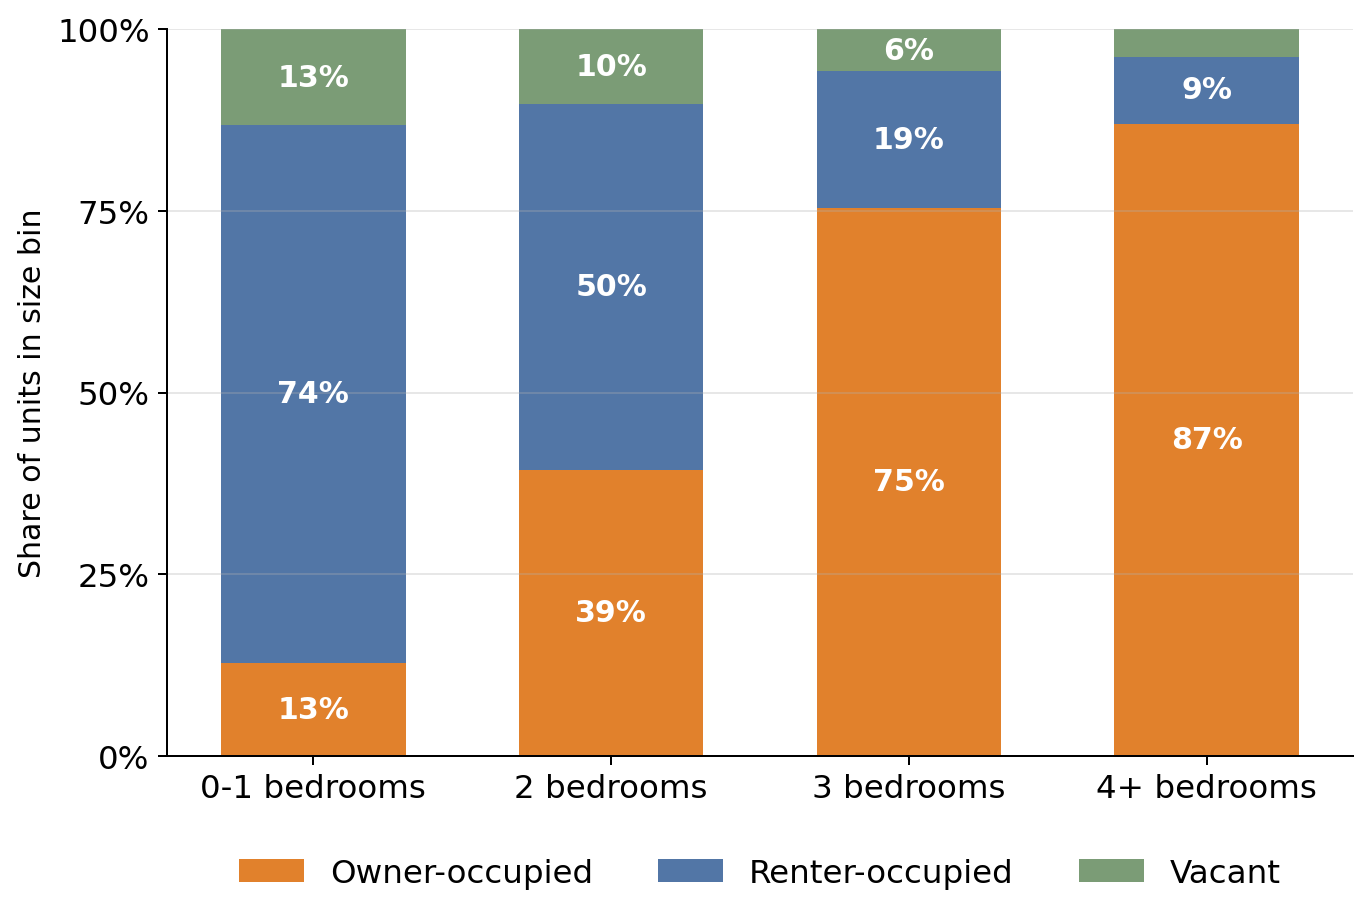
\includegraphics[width=0.62\linewidth]{ahs_tenure_share_within_size}
\caption{Tenure of the housing stock by number of bedrooms (AHS 2023)}
\label{fig:tenure-by-size}
\par\smallskip
\begin{minipage}{0.92\linewidth}
\footnotesize\textit{Notes:} Each bar divides the housing units with the
stated number of bedrooms into owner-occupied units, units rented for cash,
and vacant units. Units occupied without payment of cash rent and units whose
occupants have a usual residence elsewhere are excluded. Weighted by the
housing-unit weight. Source: American Housing Survey 2023, national
public-use file.
\end{minipage}
\end{figure}

\subsection{Who holds the large homes}

Most large owner-occupied homes are held by households without children at
home, and the largest group among them is old. Figure~\ref{fig:large-homes}
divides the owner-occupied homes with six or more rooms in 42 large
metropolitan areas in the 2023 American Community Survey (ACS) among six groups
of households, defined by the age of the householder and by whether a child of
the householder younger than 18 lives in the home. Households aged 60 to 85
without children at home hold 40.0 percent of these homes, and households
aged 40 to 59 without children at home another 21.8 percent. Households aged
22 to 39 with children hold 10.6 percent. Across all ages, 68.3 percent of the
large owner-occupied homes house no child of the householder, close to the
72.9 percent of all households in these areas without a child at home. What
the figure shows is therefore where the large homes sit by age, not that
childless households hold more than their share. I call the concentration of
large owner-occupied homes among older households the intergenerational
allocation of housing. The figure does not show that older households would
sell at some price, or that young families would have more children if they
held these homes.
% [DATA] ACS 2023 one-year, 42 metros, householders 22-85, 289,109 households;
% numbers as in the Oct 4 sandbox paper (reviewed there).
\mocktodo{name the builder of the large-homes figure in the data appendix
(not found in code/ by the Oct 4 sandbox review); the sandbox calls this
"intergenerational misallocation", which the title uses; choose the term.}

\begin{figure}[t]
\centering
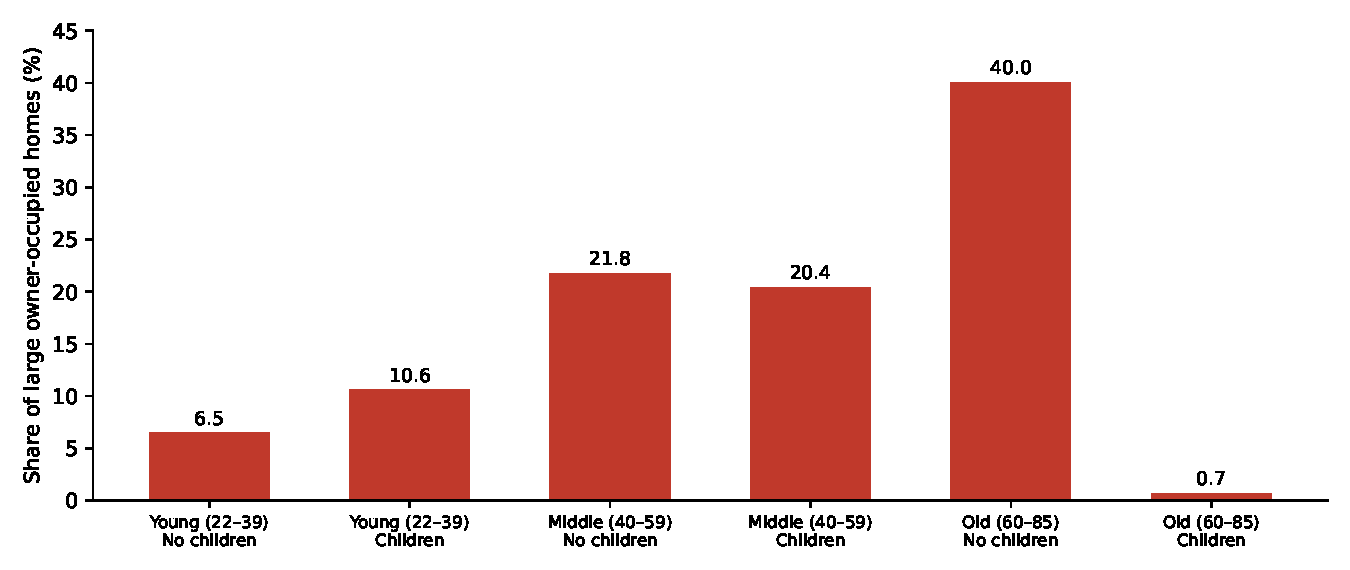
\includegraphics[width=0.9\linewidth]{large_homes_by_age_children_acs2023}
\caption{Who holds the large owner-occupied homes (ACS 2023)}
\label{fig:large-homes}
\par\smallskip
\begin{minipage}{0.92\linewidth}
\footnotesize\textit{Notes:} Each bar is the share of owner-occupied homes
with six or more rooms held by households in the group; the six shares sum to
100 percent. Groups are defined by the age of the householder and by whether
an own child of the householder younger than 18 lives in the household.
Householders aged 22 to 85 in 42 large metropolitan areas, weighted by the
household weight; 289,109 households.
\end{minipage}
\end{figure}

\subsection{Housing around the first birth}

The Panel Study of Income Dynamics (PSID) follows the same families from 1968
to 2019. I date each woman's first birth from her full history of biological
children and estimate event studies of her household's housing around it,
comparing first-time mothers with women who never have children, with the
estimator of Sun and Abraham (2021) and person and year
fixed effects. The reference window is two to three years before the birth,
so that moves made while expecting a child count as responses. The sample
keeps one woman per household and year who is its reference person or spouse.
% [DATA] mock 02_empirical_evidence.tex and data_appendix.tex; 63,338
% person-years, 3,655 first-time mothers, 1,654 childless women.

Households add about one room within four years of the first birth.
Figure~\ref{fig:emp-rooms-path} reports the path. The dwelling is 0.41 rooms
larger than in the reference window in the year of the birth, 0.82 rooms one
to two years later, and 1.03 rooms (standard error 0.07) three to four years
after it, on a base of 4.7 rooms. Fixing household position before the birth,
which removes a pre-trend that reflects who heads a household, the increase at
three to four years is 1.47 rooms (0.05). The added space comes with a move
into ownership, after which families move less (Figure~\ref{fig:emp-tenure-moves}).
The ownership rate is 11 percentage points higher in the birth window and 16
points higher three to four years later, on a base of 41 percent. The
probability of having moved since the previous interview falls by 16 to 21
points after the birth and stays lower for a decade, and among those who do
move, the share moving for more space doubles, from 12 to about 25 percent.
The ACS shows the same pattern at a point in time: among household heads aged
30 to 55, those whose oldest child is under four are 12.8 percentage points
more likely to own than heads without children.
% [DATA] ACS 2005-06 recent-parent gap 0.12761 (same as Section 4 target).

\begin{figure}[t]
\centering
\includegraphics[width=0.88\linewidth]{first_birth_rooms_psid}
\caption{Rooms around the first birth (PSID)}
\label{fig:emp-rooms-path}
\par\smallskip
\begin{minipage}{0.92\linewidth}
\footnotesize\textit{Notes:} Interaction-weighted event-study estimates in
two-year windows of event time, with 95 percent confidence intervals from
standard errors clustered by person. One woman per household-year who is the
reference person or spouse; 63,338 person-years, 3,655 first-time parents and
1,654 childless women. The hollow marker is the omitted reference window,
years $-3$ and $-2$. Mean rooms in the reference window: 4.70.
\end{minipage}
\end{figure}

\begin{figure}[t]
\centering
\includegraphics[width=0.92\linewidth]{first_birth_tenure_moves_psid}
\caption{Ownership and moving around the first birth (PSID)}
\label{fig:emp-tenure-moves}
\par\smallskip
\begin{minipage}{0.92\linewidth}
\footnotesize\textit{Notes:} Same sample, estimator and reference window as
Figure~\ref{fig:emp-rooms-path}. ``Moved for more space'' equals one if the
household moved since the previous interview and gave more space as the first
reason. Means in the reference window: ownership 0.41, moved 0.58.
\end{minipage}
\end{figure}

Figure~\ref{fig:emp-move-reasons} splits moves by the reason the household
gives. The annual probability of moving for more or better housing rises by
about 2.5 percentage points in the year before and the year of the birth and
returns to its earlier level within about five years. Moves for the
neighborhood, schools or proximity do not change around the birth. The
response to the first child is a demand for space, not for location.

\begin{figure}[t]
\centering
\begin{minipage}{0.48\linewidth}\centering
{\small Expansion or better housing}\par\smallskip
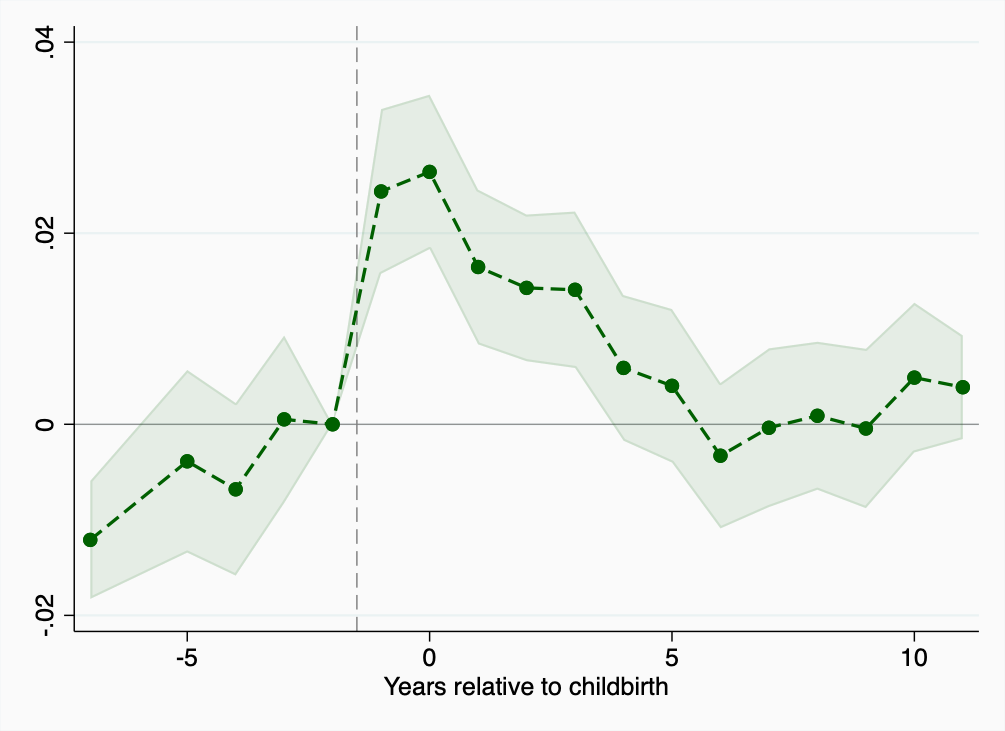
\includegraphics[width=\linewidth]{../JMP_slides/assets/mv_s_f_c_y_all.png}
\end{minipage}\hfill
\begin{minipage}{0.48\linewidth}\centering
{\small Neighborhood, schools, or proximity}\par\smallskip
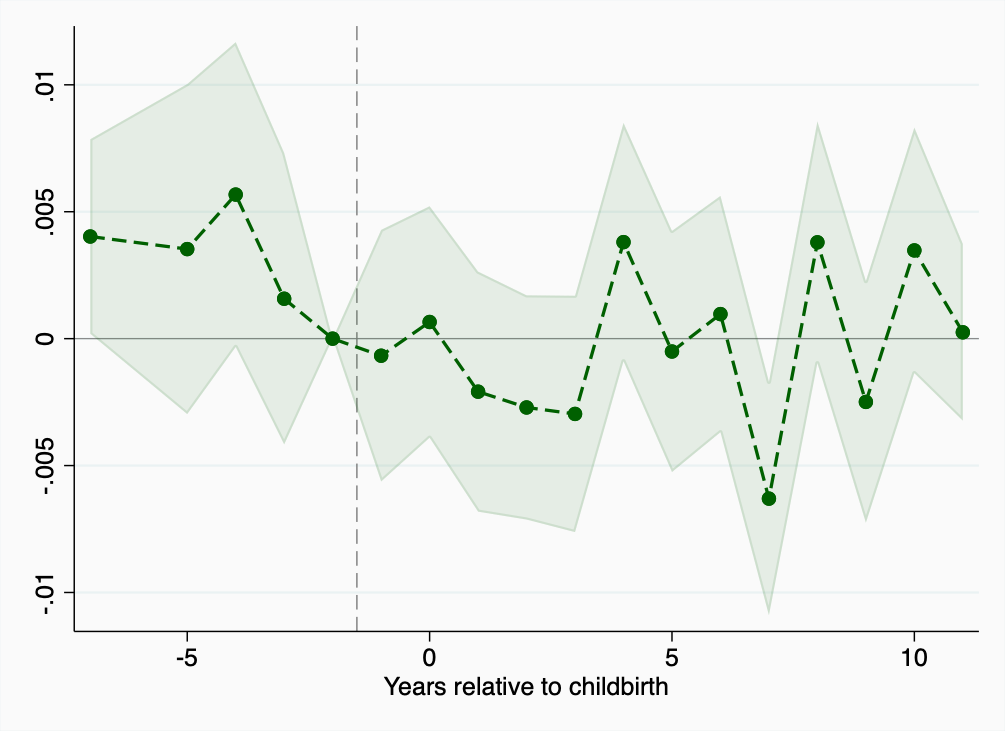
\includegraphics[width=\linewidth]{../JMP_slides/assets/mv_n_f_c_y_all.png}
\end{minipage}
\caption{Reasons for moving around the first birth (PSID)}
\label{fig:emp-move-reasons}
\par\smallskip
\begin{minipage}{0.92\linewidth}
\footnotesize\textit{Notes:} Event-study estimates of the probability of a move
for the stated reason, relative to the reference window, from the May
specification of the PSID event study.
\mocktodo{these are the deck's May estimates; the rooms and tenure figures
above are the September estimates. Re-estimate the reasons on the September
sample, or say in the notes that they come from the earlier specification.}
\end{minipage}
\end{figure}

\subsection{Implications for the model}

These facts motivate the three features that set the model apart from a
life-cycle model with a generic cost of children. Because children need
space and households add it around the first birth, fertility and housing
are chosen jointly, and a family needs a minimum of space before additional
rooms raise its welfare. Because large homes are mostly owned, the model
limits the size of rental units, so a family that wants a large home must buy
it; I call this tenure segmentation. Because buying requires a down payment
accumulated by saving, the wealth of young households and its timing matter.
And because the large homes sit with older households, the price of space for
young families depends on the whole age distribution of households; the model
is an overlapping-generations economy in which one house price clears a
market shared by all ages.

% ============================================================================
% October 13, 2026 build (agent draft). Model section of the Oct 9 build,
% brought to the engine of the 7.9167 production point: the Oct 8 sale-screen
% fix (tmp/sale_screen_fix_20261008/root, household.py 541-544: a sale into
% renting is checked by the renter budget after income arrives; the legacy
% pre-income test R b + S >= 0 is off), plus a paragraph on who owns the
% rental stock and who receives estates (deck silent; structure as in KMV
% 2020 sec. 2.4). Notation as in the Oct 12 deck (model_test_new_frames.tex).
% Supply written as H = H0 P^eta with H0 = 7.352 on this scale: the engine
% writes H0_code (u P / r_bar)^eta, H0_code = 6.81993 (promotion receipt),
% u = 0.18028, r_bar = 0.16, so H0 = 6.81993 (0.18028/0.16)^0.63 = 7.352.
% At 7.9: h_P = 1.098, hbar_child_rooms = 0, owner sizes {2,...,10}
% (p7p917 executed_P.json, read Oct 12 by the evaluation thread).
% ============================================================================
\providecommand{\mocktodo}[1]{\textcolor{red}{[TODO: #1]}}

\section{Model}
\label{sec:model}

Motivated by these observations, I build a life-cycle model in which the same
households choose when to have children, how much housing to occupy, and
whether to rent or own it. Households live in an overlapping-generations
economy, face persistent earnings risk, and save in a single bond. Children
raise the household's needs for consumption and, above all, for space. Space
can be rented or bought. A room costs the same per period whether it is
rented or owned, but the largest dwellings are available only to owners,
owners enjoy their home somewhat more, selling a home is costly, and buying
one requires a down payment, which the household pays out of its wealth and
the income of the period. House prices and rents are determined in
equilibrium by an upward-sloping supply of housing. The government runs a pay-as-you-go pension system and taxes
property, and it returns the property-tax revenue to households as an equal
transfer.

\subsection{Environment}

Time is discrete and a period lasts four years. I describe the households,
their preferences, earnings, housing, the financial market and the
government in turn.

\subsubsection*{Demographics.}
A household enters the economy at age 18 and lives at most through age 85.
Let $a$ index its age, $a_R$ the age of retirement, 66, and $J$ the last age.
It works until $a_R$ and then receives a pension. From retirement on, it
survives from one period to the next with probability $s_a<1$; before
retirement $s_a=1$.
% [MODEL INPUT] ages 18,22,...,82 (17 cells), retirement at cell 12 (age 66),
% survival 0.9391, 0.9185, 0.8850, 0.8300 for cells 12-15, certain death after
% age 82.
\mocktodo{name the source of the survival probabilities (not documented in the
repository).}
Each household is one decision unit; I do not model the formation or
dissolution of couples.

Let $n_t$ denote the number of children ever born to the household and $m_t$
the number currently living at home. Births are possible from 18 through
age 45, at most one per period. Each child at home leaves independently with
probability $\lambda$ per period, so that a child stays on average
$1/\lambda$ periods; departure lowers $m_t$ but not $n_t$. I keep track of
$n_t$ up to three, with the last state standing for three or more. Children
are dependents: they do not work and do not make decisions.
% [MODEL INPUT] fertile cells ages 18-42 (decision at the start of each
% four-year period, so births up to age 45); lambda = 2/9 per period, mean stay
% 18 years; top state n = 3 = "3+".

\subsubsection*{Preferences.}
A household values consumption $c_t$, housing services $\hat h_t$, and
children at home. Its flow utility is
\begin{equation}
 u_t(c_t,\hat h_t;m_t)
 =\frac{1}{1-\sigma}\left(\frac{c_t^{\alpha_0}\,\hat h_t^{\,1-\alpha_0}}{e(m_t)}\right)^{1-\sigma}
 +v(m_t),\qquad v(m_t)=\psi_t\, m_t^{1-\gamma}.
 \label{eq:m-utility}
\end{equation}
The first term is utility from the consumption--housing composite per
equivalent adult. The equivalence scale
\begin{equation}
 e(m_t)=\left(\frac{2+\omega\, m_t}{2}\right)^{\nu}
 \label{eq:m-escale}
\end{equation}
measures how many adult equivalents the household contains relative to a
childless couple, so that the same spending buys less utility per person in a
larger family (as in Scholz, Seshadri and Khitatrakun, 2006); it depends on
the children at home, $m_t$, not on the children ever born. The second term,
$v(m_t)$, is the direct benefit of children at home, with $\psi_t>0$ its
level and $\gamma\in[0,1)$ the rate at which the benefit of an additional
child declines.
% [CODE] shared.py 290-312: c_bar = 0 under eqscale, escale =
% (((2+0.7 m)/2)^0.7)^(sigma-1) with m = children at home (cs), which is
% e(m)^(sigma-1), the multiplier that makes u(x/e) = e^(sigma-1) x^(1-sigma)/(1-sigma);
% child_preferences.py 31-33: benefit = psi_child m^(1-curvature) for m >= 1. The level $\psi_t$
carries a time subscript because it is the object that changes in the
historical exercise of Section~\ref{sec:quant-transition}. Becoming a parent
carries, in addition, a one-time utility cost $\xi$ at the first birth.

Children need room. A household with children at home obtains services only
from the space in excess of a minimum $\bar h(m_t)=h_P\,\1\{m_t>0\}$:
\begin{equation}
 \hat h_t=
 \begin{cases}
 h^R_t-\bar h(m_t), & \text{renter of } h^R_t \text{ rooms},\\[2pt]
 \chi\bigl[h_t-\bar h(m_t)\bigr], & \text{owner of } h_t \text{ rooms},
 \end{cases}
 \qquad \chi>1 .
 \label{eq:m-services}
\end{equation}
The parenthood space requirement $h_P$ is the space a family needs before
additional rooms add to its welfare. It is measured in rooms and does not
depend on the number of children, so it is the first child that creates the
need for space. The owner multiplier $\chi$ captures the additional services
an owner obtains from a dwelling of a given size, for example from the
ability to adapt it, and applies only to the rooms above the requirement. A
household with children in a dwelling of $h_P$ rooms or fewer obtains
essentially no housing services, so in practice parents occupy more than
$h_P$ rooms, whether they rent or own.
% [CODE] owner services chi*(h - h_P) (kernels.py 922-931: ht_c = hsv -
% owner_h_bar_scale*hbc, clamped at 1e-10 when h <= h_P, then times
% owner_service_premium; strict_hbar_feasibility is never passed, so the
% option is dominated, not infeasible). Renter: rent on h_P is paid first,
% dc = cbc + ri*hbc, and ht_unc = (1-al)*surplus/ri (kernels.py 726-729,
% 833-855). h_bar = hbar_first_child_jump + hbar_child_rooms*m (shared.py
% 291-296). The deck's "Utility Specification" frame writes
% chi[h - hbar(m)] + [h^R - hbar(m)] as one expression; read tenure by tenure,
% it is (eq:m-services).
Together, \eqref{eq:m-utility} and \eqref{eq:m-services} define what a child
costs. At given prices, a first child raises the spending needed to reach a
given utility in two ways: through the equivalence scale, which scales up all
spending, and through the space requirement, which must be paid at the rent
of a room before any housing yields services. The second part is paid every
period the child is at home, by renters and owners alike.

\subsubsection*{Fertility.}
At the start of each fertile period, a household chooses whether to try for a
child. An attempt succeeds with probability $\pi_a$, which declines with age,
and adds one child: $n_{t+1}=n_t+1$. The decision is subject to type-I
extreme-value taste shocks $\varepsilon^F_t$ with scale $\kappa_1$ when the
household is childless and $\kappa_C$ when it already has children, so that
childlessness and family size can respond differently to the same change in
incentives. After the outcome of the attempt is known, the household chooses
its housing and saving for the period. Housing can therefore adjust to a
birth within the same period, which matches the timing of the room response
in Section~\ref{sec:empirical-evidence}.
% [MODEL INPUT] pi_a = 1 - 0.02 exp(0.134 (age - 18)), zero from 45
% (parameters.py 21-45).
% [CODE] household.py 1000-1016: V = birth_count_menu(VI, n, m, pi_j,
% kappa_fert if n == 0 else kappa_fert_continuation, first_birth_fixed_cost,
% cap = 1), where VI is the housing/saving value after the birth outcome;
% birth_count.py 46-84: with cap 1 the menu is {wait, attempt} and the
% attempt value is pi*(VI[n+1,m+1] - xi*1{n=0}) + (1-pi)*VI[n,m], which is
% (eq:m-wait-attempt) and (eq:m-attempt).

\subsubsection*{Firms and earnings.}
Competitive firms produce with effective labor, $Y_t=A L_t$, where
$L_t=\int_{a<a_R} e_a z_t\,\dd G_t$ and $G_t$ is the distribution of
households over states, so the wage per efficiency unit is $w=A$, which I
normalize to one. Before retirement, a household of age $a$ earns, after the
payroll tax,
\begin{equation}
 y^d_t(a,z_t)=(1-\tau^w)\,w\,e_a\,z_t ,
 \label{eq:m-earnings}
\end{equation}
where $e_a$ is a deterministic age profile and $z_t$ an idiosyncratic labor
efficiency. Efficiency follows a first-order autoregressive process in logs,
\begin{equation}
 \log z_{t+1}=(1-\rho_z)\mu_z+\rho_z\log z_t+\epsilon_{t+1},\qquad
 \epsilon_{t+1}\sim N(0,\sigma_z^2),
 \label{eq:m-ar1}
\end{equation}
where $\mu_z$ normalizes mean efficiency to one. Earnings risk is the only
source of income uncertainty. From $a_R$ on, every retiree receives the same
pension $\varpi_t$.
% [MODEL INPUT] rho_z = 0.735, sigma_z = 0.484 per four-year period; nine
% states; pension flat.
% [CODE] e5f_social_security.py 40-41: income[:, :J_R] = (1-tax)*wage*profile,
% retirees receive the pension; shared.py 114-131: income_at_state = y*z before
% retirement, the flat pension after (retirement_income_z_scale = 0), plus the
% rebate at every age.
\mocktodo{name the data source of the age profile $e_a$ (not documented in
the files read).}

\subsubsection*{Housing and tenure.}
Housing is measured in rooms and trades at price $P_t$ per room. An owner
lives in a house of $h_t\in\mathcal H=\{2,4,6,8,10\}$ rooms. A renter rents
any $h^R_t\in[0,\bar h^R]$ rooms at rent $r_t$ per room, with
$\bar h^R<\max\mathcal H$, so the largest dwellings are reachable only
through ownership, as in the American Housing Survey facts of
Section~\ref{sec:empirical-evidence}. I call this tenure segmentation. Owners
pay depreciation $\delta_H$ and property tax $\tau^p_t$ on the value of their
home each period. Selling a home costs a fraction $\psi^s$ of its value;
buying costs nothing beyond the price. The tenure and dwelling choice is
subject to type-I extreme-value taste shocks $\varepsilon^H_t$ with scale
$\kappa_T$, one for each option: renting, keeping the current home, or buying
each size in $\mathcal H$.
% [CODE] household.py 194-206: hcost = P h, heq = (1-psi) P h, ocst =
% (delta + tau_H) P h, dp = (1-phi) P h, bmo = -phi P h; kernels.py 383-474
% (tenure_logit_kernel): options tn = 0 rent, tn >= 1 own size tn, with the
% stay value used when tn equals the current size.

\subsubsection*{Rents and housing supply.}
Competitive landlords own the rental stock. A landlord buys a room at $P_t$,
pays depreciation and property tax, rents it out at $r_t$, and sells it at
$P_{t+1}$. Landlords finance themselves at the household bond return $R_b$,
so zero profits require that rent equal the user cost of housing,
\begin{equation}
 r_t=(R_b+\delta_H+\tau^p_t)P_t-P_{t+1},
 \qquad\text{and in a steady state}\qquad
 r=(R_b-1+\delta_H+\tau^p)P .
 \label{eq:m-rent}
\end{equation}
Because rent equals the user cost and households and landlords borrow and
save at the same rate, a room costs the same per period whether it is rented
or owned. Tenure matters for the cost of a family through four features
only: the size limit on rentals $\bar h^R$, the owner multiplier $\chi$, the
cost of selling $\psi^s$, and the down payment described next. Along a
transition, \eqref{eq:m-rent} prices rent net of the expected capital gain,
so when the price is expected to recover, rent lies below the static user
cost.
Three ownership conventions close the housing block. The rental stock
belongs to landlords outside the household sector: they hold rooms at zero
profit, financed at the bond return, so rent income does not accrue to any
household in the model. New rooms are produced by builders who are also
outside the household sector, so construction revenue is not household
income. And estates are not inherited by other households (see Bequests
below). These are the conventions of Kaplan, Mitman and Violante (2020,
Section 2.4).\footnote{The conventions matter for the policy comparisons. The
revenue of builders and the return of landlords leave the household sector,
so a supply expansion or a rise in the house price does not feed back into
household income. A closed version of the economy would return them to
households, for example as dividends.}
% [CODE] steady state: inputs.py 159, user_cost_rate = (R_gross - 1) + delta
% + tau_H = 0.18028 per period; equilibrium.py 641, r = user_cost_rate * p.
% The dated rule along a transition is implemented in the transition runner,
% which is not in the engine files reviewed; it is stated as in the deck.

Housing is supplied by a competitive construction sector with a constant
elasticity with respect to the price,
\begin{equation}
 H^s_t=H_0\,P_t^{\eta},
 \label{eq:m-supply}
\end{equation}
where $H_0$ sets the scale of the stock and $\eta$ is the supply elasticity.
In the baseline, the stock is on this curve at every date: it adjusts to the
price within a period. Appendix~\ref{app:policy-more} reports the
policy experiments with the stock held fixed at its 2023 level.
% [MODEL INPUT] eta = 0.63; H0 = 7.352 on this scale at 7.9 (engine: H0_code
% 6.820 on the scale (u P / 0.16)^eta).
% [CODE] distribution.py 3213-3223 and 3256-3257, native_phase_b.py 97-99:
% supply = H0 * (user_cost_rate * p / r_bar) ** xi_supply, xi_supply = 0.63,
% r_bar = 0.16; demand = renter rooms + owner rooms. H0 = 6.312 *
% (0.18028/0.16)^0.63 = 6.805. inputs.py: eta_supply = 1.75 is an unused
% field; the elasticity in the law is xi_supply.

\subsubsection*{Saving and mortgages.}
Households save in a one-period bond $b_{t+1}$ with gross return $R_b$, fixed
in the world market; $b_{t+1}<0$ is mortgage debt. Borrowing must be secured
by a home: a renter cannot borrow, $b_{t+1}\geq0$. At origination, a buyer
must put down at least a fraction $1-\phi$ of the price,
\begin{equation}
 b_{t+1}\geq-\phi\,P_t h_t ,
 \label{eq:m-ltv}
\end{equation}
and afterwards the house is collateral for an owner who stays,
$b_{t+1}\geq\min\{b_t,-\phi P_t h_t\}$: a stayer pays the interest on its
mortgage and does not borrow more. An owner whose debt exceeds
$\phi P_t h_t$ after a fall in the price is therefore not forced to repay,
but cannot borrow more. The down payment is paid out of the wealth the
household brings into the period and the income it earns during it. With the
budget constraint below, \eqref{eq:m-ltv} makes a purchase feasible when
$R_b b_t+y^d_t+T_t\geq(1-\phi)P_t h_t$, so a household with little wealth
can buy out of a period's income, and there is no separate rule for how the
down payment is financed. One further restriction keeps estates
nonnegative: from retirement on, when the household may die, its debt may not
exceed the sale value of its home net of the selling cost,
$b_{t+1}\geq-(1-\psi^s)P_t h_t$. An owner who sells and returns to renting
faces the renter's budget and borrowing limit, with the net proceeds of the
sale and the period's income both available, so a sale is possible whenever
$R_b b_t+(1-\psi^s)P_t h_{t-1}+y^d_t+T_t$ covers the rent and consumption.
Mortgages carry no amortization schedule and no limit on payments relative
to income.
% [CODE] renter floor: household.py 47-58 (unsecured_credit_limit = 0, so
% b' >= 0). Origination: household.py 205-206 (dp = (1-phi) P h, bmo =
% -phi P h), kernels.py 955-959 (total_floor = bf + unsecured_floor, with the
% unsecured part zero); phi = 0.80. Down payment from post-interest wealth
% plus income: household.py 926-931, dp_choice = (dp_arr - income)/R and
% bmo_purchase = (bmo - income)/R; kernels.py 433-445, a buyer from renting
% is infeasible if b < dp_choice or b - P h/R < bmo_purchase, both of which
% read R b + y >= (1-phi) P h (income includes the rebate, shared.py
% 114-131). Stayer: kernels.py 976-979, total_floor = max(min(b, -phi P h),
% due_death_floor); household.py 61-72. Net-estate floor: household.py
% 40-44, -(1-psi) P h when death_possible_at_age (household.py 33-38: last
% cell or survival < 1, so from the retirement cell on); kernels.py 980-983
% applied to buyers and stayers. Sale solvency: kernels.py 417-420, selling to
% rent is infeasible if R b + (1-psi) P h < 0 (require_owner_sale_solvency;
% credit.py 5-19). A seller who rebuys needs R b + (1-psi) P h_old + y >=
% (1-phi) P h_new (kernels.py 447-451). Oct 13: at 7.9 the sale-to-rent test is
% the renter budget after income (household.py 541-544, sale_screen_fix root;
% require_owner_sale_solvency only under legacy_pre_income_sale_screen, off).
% No amortization, no PTI
% (household.py 729-742 forbid them with native_purchase_income).

\subsubsection*{Budget constraint.}
Transactions in housing take place after interest accrues on the bond carried
into the period. A household that enters with $h_{t-1}$ owned rooms (zero for
a renter) and leaves with $h_t$ owned rooms and $h^R_t$ rented rooms faces
\begin{equation}
 c_t+b_{t+1}+r_t h_t^R+(\delta_H+\tau_t^p)P_t h_t
 =R_b b_t+y_t^d(a,z_t)+T_t-\1\{h_t\neq h_{t-1}\}\,P_t\bigl[h_t-(1-\psi^s)h_{t-1}\bigr],
 \label{eq:m-budget}
\end{equation}
where $y^d_t$ is earnings after the payroll tax or the pension and $T_t$ is
the lump-sum transfer from the government. A renter has $h_t=0$, an owner
$h^R_t=0$, and a household that keeps its home pays no transaction. The sale
proceeds and the purchase price are not compounded: a household that sells
and buys within a period carries only the difference into next period's
interest.
% [CODE] post-interest timing (author-adopted Oct 3): household.py 317,
% Rv = R b + y with y including the rebate; kernels.py 417 (sale to rent, b +
% (1-psi) P h/R), 433 (purchase, b - P h/R), 447 (sell and rebuy, b +
% ((1-psi) P h_old - P h_new)/R), so transactions are added to the bond after
% interest and carried into next period's interest only as a net amount.
% Owner cost (delta + tau_H) P h each period: household.py 200.

\subsubsection*{Bequests.}
A household that dies leaves its estate net of the selling cost,
$w^e_{t+1}=b_{t+1}+(1-\psi^s)P_t h_t$, and values it according to
\begin{equation}
 B(w^e_{t+1})=\theta_0\,\frac{(\theta_1+w^e_{t+1})^{1-\sigma}}{1-\sigma},
 \label{eq:m-bequest}
\end{equation}
where $\theta_0$ governs the strength of the bequest motive and $\theta_1$
the extent to which bequests are a luxury.%
\footnote{The estate enters $B$ as $\max\{w^e_{t+1},0\}$. Under the
borrowing constraints above it is nonnegative at every age at which death is
possible, so the truncation never binds.}
Estates are not received by other households; entrants' wealth is drawn from
the data instead, as described below.
% [CODE] Estate A: household.py 845-856, Vbq = bequest_utility_vec(b' + hv)
% with hv = (1-psi) P h (bequest_utility_net_active); household.py 1548-1582,
% b = max(b, 0), scale theta0*(1 + theta_n nk) with theta_n = 0, utility
% (theta1 + b)^(1-sigma)/(1-sigma), the zero-estate normalization only if
% normalize_bequest_utility (default False; the earlier footnote claiming the
% engine subtracts theta0 theta1^(1-sigma)/(1-sigma) could not be verified
% and was removed). No estate tax, estate_receiver = 'none'. Death branch:
% household.py 868-869 (last cell) and 879-881, Vnr = s*Vnr + (1-s)*Vbq.

\subsubsection*{Government.}
The government runs two programs, each with a balanced budget in every
period. The pension system pays every retiree the same pension $\varpi_t$,
financed by the payroll tax $\tau^w$ on earnings. The property tax raises
$\tau^p_t$ times the value of the entire housing stock, owned and rented:
owners pay it directly, and renters pay it through the rent, into which the
landlord passes it by \eqref{eq:m-rent}. Its revenue is returned to all
households, of every age and tenure, as an equal lump-sum transfer $T_t$, the
rebate.
% [CODE] shared.py 595-610: revenue = tau_H * price * (rental rooms + owner
% rooms); fiscal_closure.py 59-69: T*N = revenue - grants, equal lump sum at
% all ages (property_tax_rebate_closure = 'balanced'); shared.py 114-131 adds
% T to income at every age. Pension: e5f_stationary_paygo.py 47-62 solves the
% flat pension that balances the payroll tax given the exogenous age-income
% mass; e5f_social_security.py 50-96 certifies the balance (PAYGO_TOL 1e-6).

\subsubsection*{Entry.}
Households enter at age 18 as childless renters. Each entrant draws its
efficiency from the stationary distribution of $z$. Its wealth comes from the
distribution of net worth among childless renters aged 18 to 24 who head their
household in the PSID, 1984 to 2019, with negative net worth set to zero.
Dollar amounts are converted to model units with one common scale, chosen so
that mean income in this sample equals mean earnings of entrants in the
model, and observations are assigned to efficiency states by income rank, so
that the poorest entrants in the data become the least productive entrants in
the model. The children born in the model form the entering households: the
number of entrants in each period equals the number of children born sixteen
and twenty years earlier, half from each cohort, divided by 2.1, so that the
population is constant when each household has 2.1 children on average.
% [CODE] adult_entry.py 14-32: entry = adjusted births / 2.1, where a birth
% into the top state n = 3 counts tfr_top_bin_weight = 3.602 children;
% native_phase_b.py 265-270 and distribution.py 1446-1457: split queue, half
% due 16 years after birth (4 periods) and half 20 (5 periods).
% distribution.py 597-613: entrants are childless renters at the first cell,
% z drawn from z_weights, wealth from the PSID law. entry_wealth.py 197-293:
% levels_rank law, negative net worth censored at zero, one scale lambda =
% model mean annual gross entry earnings (transfers excluded) / weighted mean
% sample family income, exact weighted income-rank allocation to z states.

\subsection{The household's problem}
\label{sec:m-household}

The state of a household at the start of a period is its age $a$, bond
position $b_t$, housing $h_{t-1}$, efficiency $z_t$, and children $n_t$ and
$m_t$. A period has two stages. The household first sees its fertility taste
shocks and decides whether to attempt a birth. It then learns whether the
attempt succeeded, sees its tenure taste shocks, and chooses tenure,
dwelling, consumption and saving. Children leave home and efficiency is drawn
between periods.

\subsubsection*{Housing and saving.}
After the birth outcome, the value of the household is
\begin{multline}
 V^H_t(b_t,h_{t-1},z_t,a,n,m)
 =\E_{\varepsilon_t^H}\max_{h_t,h_t^R,b_{t+1}}
 \Bigl\{u_t\big(c_t,\hat h_t;m\big)+\varepsilon_t^H(h_t)\\
 +\beta\,\E_t\Bigl[s_a V_{t+1}(b_{t+1},h_t,z_{t+1},a+1,n,m_{t+1})
 +(1-s_a)B(w^e_{t+1})\Bigr]\Bigr\}
 \label{eq:m-vh}
\end{multline}
subject to the budget constraint \eqref{eq:m-budget}, the services
\eqref{eq:m-services}, and the borrowing constraints: $b_{t+1}\geq-\phi
P_th_t$ for a household that buys or rents, $b_{t+1}\geq\min\{b_t,-\phi
P_th_t\}$ for an owner who stays, and, when death is possible,
$b_{t+1}\geq-(1-\psi^s)P_th_t$. The expectation is over next period's
efficiency $z_{t+1}$ and the number of children $m_{t+1}$ still at home. An
option is available only if it leaves room for a saving choice that
satisfies the borrowing constraints, and a sale only if the net proceeds
repay the mortgage. Given the option $o$ (renting, keeping
the home, or buying each size), let $V^o_t$ denote the value of the best
choice of $c_t$, $h^R_t$ and $b_{t+1}$. With the extreme-value shocks,
\begin{equation}
 V^H_t=\kappa_T\log\sum_{o}\exp\bigl(V^o_t/\kappa_T\bigr),
 \qquad
 \pi^H_{t,a}(o)=\frac{\exp(V^o_t/\kappa_T)}{\sum_{o'}\exp(V^{o'}_t/\kappa_T)} .
 \label{eq:m-tenure}
\end{equation}
Because the composite in \eqref{eq:m-utility} is Cobb--Douglas, a renter not
at the size limit spends a share $1-\alpha_0$ of its outlay net of the space
requirement on rooms above $h_P$.
% [CODE] kernels.py 383-474 (tenure_logit_kernel): VH = best_v +
% kappa*log(sum exp((V^o - best_v)/kappa)) over the feasible options, which is
% (eq:m-tenure); kernels.py 833-855: renter ht_unc = (1-al)*surplus/ri, capped
% at hR_max - h_bar.

\subsubsection*{Fertility.}
Before the birth outcome, a household with $n_t<3$ in a fertile period
compares waiting and attempting, with values
\begin{equation}
\begin{aligned}
 W_t^0&=V^H_t(b_t,h_{t-1},z_t,a,n_t,m_t),\\
 W_t^A&=\pi_a\Bigl[V^H_t(b_t,h_{t-1},z_t,a,n_t+1,m_t+1)-\xi\,\1\{n_t=0\}\Bigr]
 +(1-\pi_a)\,V^H_t(b_t,h_{t-1},z_t,a,n_t,m_t).
\end{aligned}
 \label{eq:m-wait-attempt}
\end{equation}
With scale $\kappa(n_t)=\kappa_1$ if $n_t=0$ and $\kappa_C$ otherwise, the
value at the start of the period is
\begin{equation}
 V_t(b_t,h_{t-1},z_t,a,n_t,m_t)
 =\E_{\varepsilon_t^F}\max\bigl\{W_t^0+\varepsilon^F_{t,0},\;W_t^A+\varepsilon^F_{t,A}\bigr\},
 \label{eq:m-fertility}
\end{equation}
and the probability of attempting a birth is
\begin{equation}
 \pi^F_{t,a}(b_t,h_{t-1},z_t,n_t,m_t)
 =\frac{\exp\{W_t^A/\kappa(n_t)\}}{\exp\{W_t^A/\kappa(n_t)\}+\exp\{W_t^0/\kappa(n_t)\}} .
 \label{eq:m-attempt}
\end{equation}
Outside the fertile ages, or with $n_t=3$, $V_t=V^H_t$. A birth is therefore
attempted when the value of the household with one more child, net of the
cost of becoming a parent, exceeds the value of waiting by enough to overcome
the taste shocks. Anything that changes the resources a household can devote
to the space a child requires, or the risk around them, changes the gap
$W^A_t-W^0_t$ and with it the probability of a birth.

\subsection{Equilibrium}
\label{sec:m-equilibrium}

Let $G_t$ be the distribution of households over states and $N_t$ the number
of households. Given parameters, an initial population $N_0$ and an initial
distribution $G_0$, an equilibrium is a sequence
$\{V_t,g_t,G_t,N_t,P_t,r_t,T_t,\varpi_t\}_{t\geq0}$ such that, at every date:
\begin{enumerate}
\item \emph{Households.} Given $\{P_{t'},r_{t'},T_{t'},\varpi_{t'}\}_{t'\geq
t}$, $V_t$ solves the household problem of Section~\ref{sec:m-household}
with continuation $V_{t+1}$, and the policy functions $g_t$ (fertility,
tenure, dwelling, consumption and saving) attain it.
\item \emph{Rents.} The rent satisfies the landlord's zero-profit condition
\eqref{eq:m-rent}.
\item \emph{Housing market.} The rooms occupied by owners and renters equal
the supply \eqref{eq:m-supply},
\[
 N_t\int\bigl[h_t+h^R_t\bigr]\dd G_t=H_0\,P_t^{\eta}.
\]
\item \emph{Government.} The pension system balances,
$\tau^w w\int_{a<a_R}e_az_t\,\dd G_t=\varpi_t\int_{a\geq a_R}\dd G_t$, and the
rebate returns the property-tax revenue,
$T_t=\tau^p_tP_t\int\bigl[h_t+h^R_t\bigr]\dd G_t$.
\item \emph{Population.} Births are $N_t\int\pi_a\pi^F_{t,a}\,\dd G_t$.
Households survive to the next age with probability $s_a$, and the children
born form new households when they reach adulthood, as described under Entry.
\item \emph{Consistency.} $G_{t+1}$ and $N_{t+1}$ follow from $G_t$ and $N_t$
under $g_t$, the shocks, survival, the departure of children and entry.
\end{enumerate}
A stationary equilibrium is an equilibrium in which prices, the pension, the
rebate and $G_t$ are constant. In a stationary equilibrium the population is
constant only if households have 2.1 children on average, so the house price
is the one at which the population reproduces itself, and the population is
the one that clears the housing market at that price. Two features of the
equilibrium are worth stating. First, the price of housing links fertility to
housing supply: more births raise the demand for rooms by families, which
raises $P_t$ and $r_t$ and with them the cost of the space a child requires.
Second, because the housing stock is durable and the population responds to
fertility only with a lag of a generation, a change in fertility moves the
price of space for decades.%
\footnote{In the calibration I normalize the 2007 population to one and set
$H_0$ so that the market clears at the price consistent with replacement. In
every counterfactual $H_0$ is held fixed and the population adjusts.}
% [CODE] production/README.md: price root = birth-renewal residual; H0
% derived under population_one, held fixed (fixed_h0) in counterfactuals.
% equilibrium.py (model) 84-96: renewal_root = adjusted_births/(2.1*entry)
% - 1, implied H0 = demand/(u P/r_bar)^xi; native_phase_b.py 25-26, 126-127:
% RENEWAL_TOL 1e-6, population = supply/demand under fixed_h0;
% distribution.py 1101-1102 (survival), 1219-1264 (child departure via
% Pi_child and entrants maturing), 1419-1430 (property-tax revenue and rebate
% outlays on the current distribution).

\subsection{A graphical illustration}
\label{sec:m-illustration}

Figure~\ref{fig:m-illustration} summarizes how the equilibrium responds to a
fall in the preference for children. Summarize housing costs by $p$ and
fertility by $n(p;\psi)$, decreasing in $p$. Panel~(a) of the top row shows
the housing market: given the adult population $S$, the housing cost
$P(S;\psi)$ clears the market. Panel~(b) shows fertility as a function of the
housing cost. At $A$, housing clears at $(S_0,p_0)$ and fertility is at the
replacement rate $\bar n$. A fall in the preference from $\psi_0$ to $\psi_1$
first lowers fertility at the unchanged housing cost, from $A$ to $A'$
(middle row). With fewer children at home, housing demand falls and the
housing cost adjusts at the inherited population $S_0$, from $A'$ to $B$.
Over the following generations, smaller entering cohorts reduce housing
demand further (bottom row). Lower housing costs partly offset the decline in
the preference, and $C$ marks the new stationary outcome, at which fertility
is again at replacement with a smaller population and cheaper housing. The
quantitative transition of Section~\ref{sec:quant-transition} follows these
steps.

\begin{figure}[p]
\centering
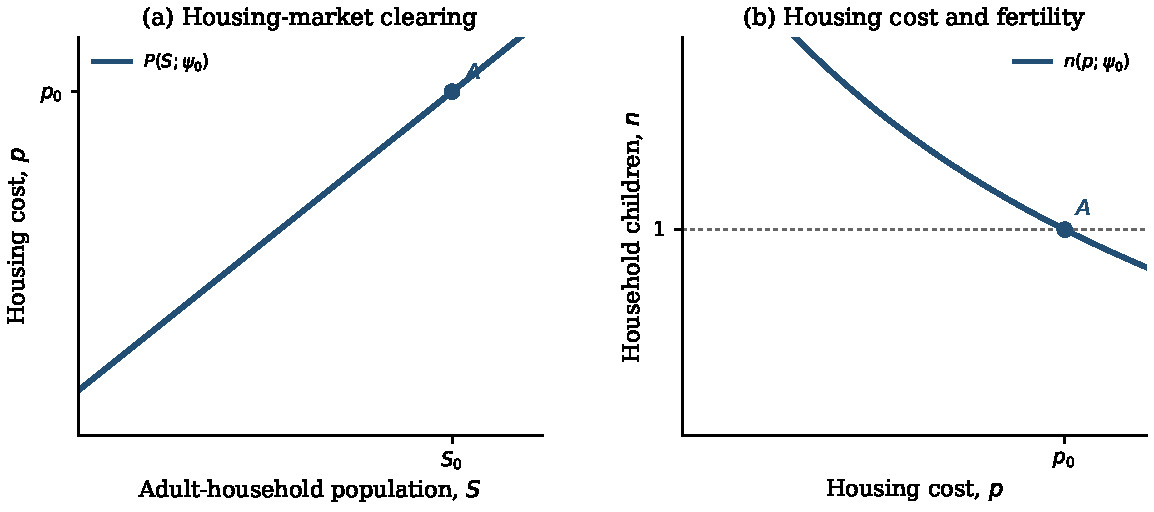
\includegraphics[width=0.86\linewidth]{september_housing_fertility_stage_initial}\\[0.4em]
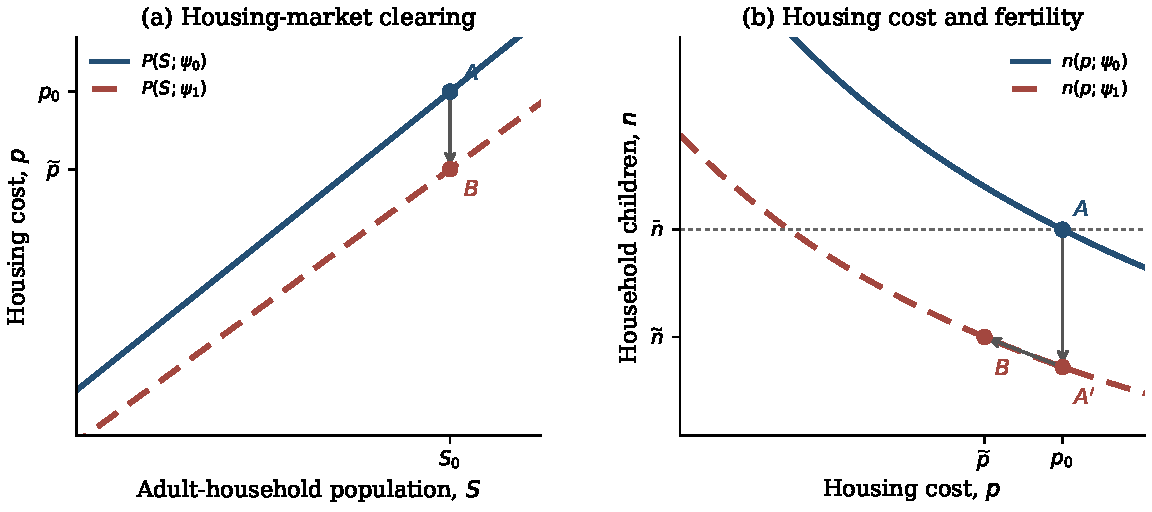
\includegraphics[width=0.86\linewidth]{september_housing_fertility_stage_impact}\\[0.4em]
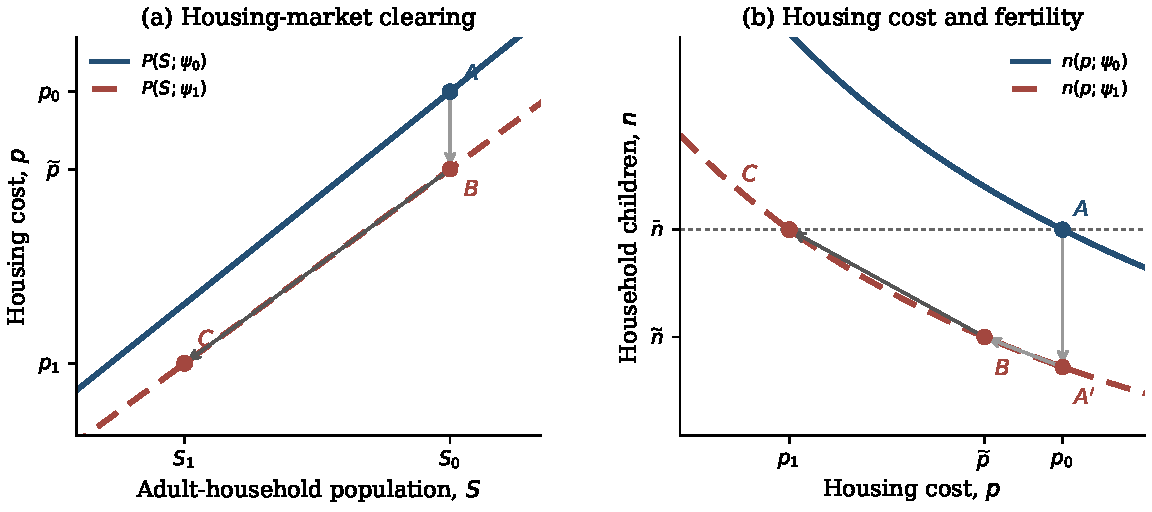
\includegraphics[width=0.86\linewidth]{september_housing_fertility_stage_adjustment}
\caption{Fertility, housing costs and population: initial steady state,
impact, and demographic adjustment}
\label{fig:m-illustration}
\par\smallskip
\begin{minipage}{0.92\linewidth}
\footnotesize\textit{Notes:} Schematic. Panel (a) of each row: housing-market
clearing; panel (b): housing cost and fertility. Top: the initial steady
state $A$. Middle: a fall from $\psi_0$ to $\psi_1$ ($A\to A'\to B$). Bottom:
demographic adjustment to the new stationary outcome $C$.
\end{minipage}
\end{figure}

% Section 4 at the recalibrated new-accounting point (loss 7.4186), Oct 21 2026.
% Parameters and 2007 fit: output/model/calibration/2026-10-19_identification_newacct/
% (torch/best_point.json; moments/center.json: target_fit, event paths, price, loss).
% Mothers by 25 and 2007 life-cycle: output/model/calibration/2026-10-21_lifecycle_newacct/
% (Results write-up thread's fixed-price 2007 solve).
% Transition (Oct 24, free entry main): FIN063fi_fw.json (eta 0.63, free entry, rho 0.35, psi_inf
% 0.148414), in output/model/experiments/housing_supply/20261022_fi_all_arms/history/.
% 2023 table and life-cycle: .../housing_supply/20261021_free_entry/moments_2023_fi/ (free_entry_eta0.63
% column; same observers as the 7.9 table, replay of the converged FIN063fi_fw history).
% Oct 25: 4.1-4.2 restructured on the model of Boar, Gorea and Midrigan (2017, Sec. 4.1, Table 2);
% Section 5 (Testing the model) is in 05_testing.tex.

\section{Quantification}
\label{sec:quant}

In this section, I describe the quantification of the model. Because
fertility rates vary a lot over time and the age distribution of the
population reflects many years of past fertility decisions, some assumptions
are needed to make the quantification tractable. To this end, I approximate
the United States economy of 2007 with a steady state in which births are at
replacement. I parameterize the model so that this steady state matches
fertility, housing and wealth moments of 2007. Holding these parameters
fixed, I then let the preference for children $\psi_t$ fall after 2007 so
that the model matches the decline in fertility until 2023, and I solve for
the transition of the economy as prices, family composition and household
entry adjust (Section~\ref{sec:quant-transition}). I treat this fall as an
exogenous shock to preferences and take it as given. The 2023 state of this
transition is the starting point of the policy experiments in
Section~\ref{sec:policy}.

\subsection{Quantification strategy}
\label{sec:quant-approach}

Two measures of fertility guide the quantification
(Figure~\ref{fig:quant-us-fertility}). Period fertility, or the total
fertility rate, is the number of children a woman would have if she lived
through her fertile years at the birth rates of a given year. Completed
fertility is the number of children a woman has had by the end of her fertile
years. I measure it at ages 40 to 44. Whether a population replaces itself
depends on completed fertility, which is then the key number to look at when thinking about population growth trends. In a steady state the two measures coincide. Out of
a steady state, completed fertility lags period fertility, because it adds up
the births of a cohort over two decades. In the United States, period
fertility peaked at about 2.1 in 2007 and fell to 1.62 by 2023, while
completed fertility was still 1.92 in 2024. If period fertility stayed at its
2023 level, completed fertility would fall to 1.62 within about two decades,
as the cohorts that had their children before 2007 age out.\footnote{The
same lag explains why the number of households does not fall at once when
fertility falls: fewer births lower the number of new households only when
the smaller cohorts reach adulthood. This is also why, despite almost two
decades of below-replacement period fertility, the population of the United
States has not yet started to decrease.}
% Model: households 1.000 through the period dated 2019, 0.997 in 2023, 0.989 in 2027
% (FIN063fi_fw.json rows adult_population).

\begin{figure}[!htbp]
\centering
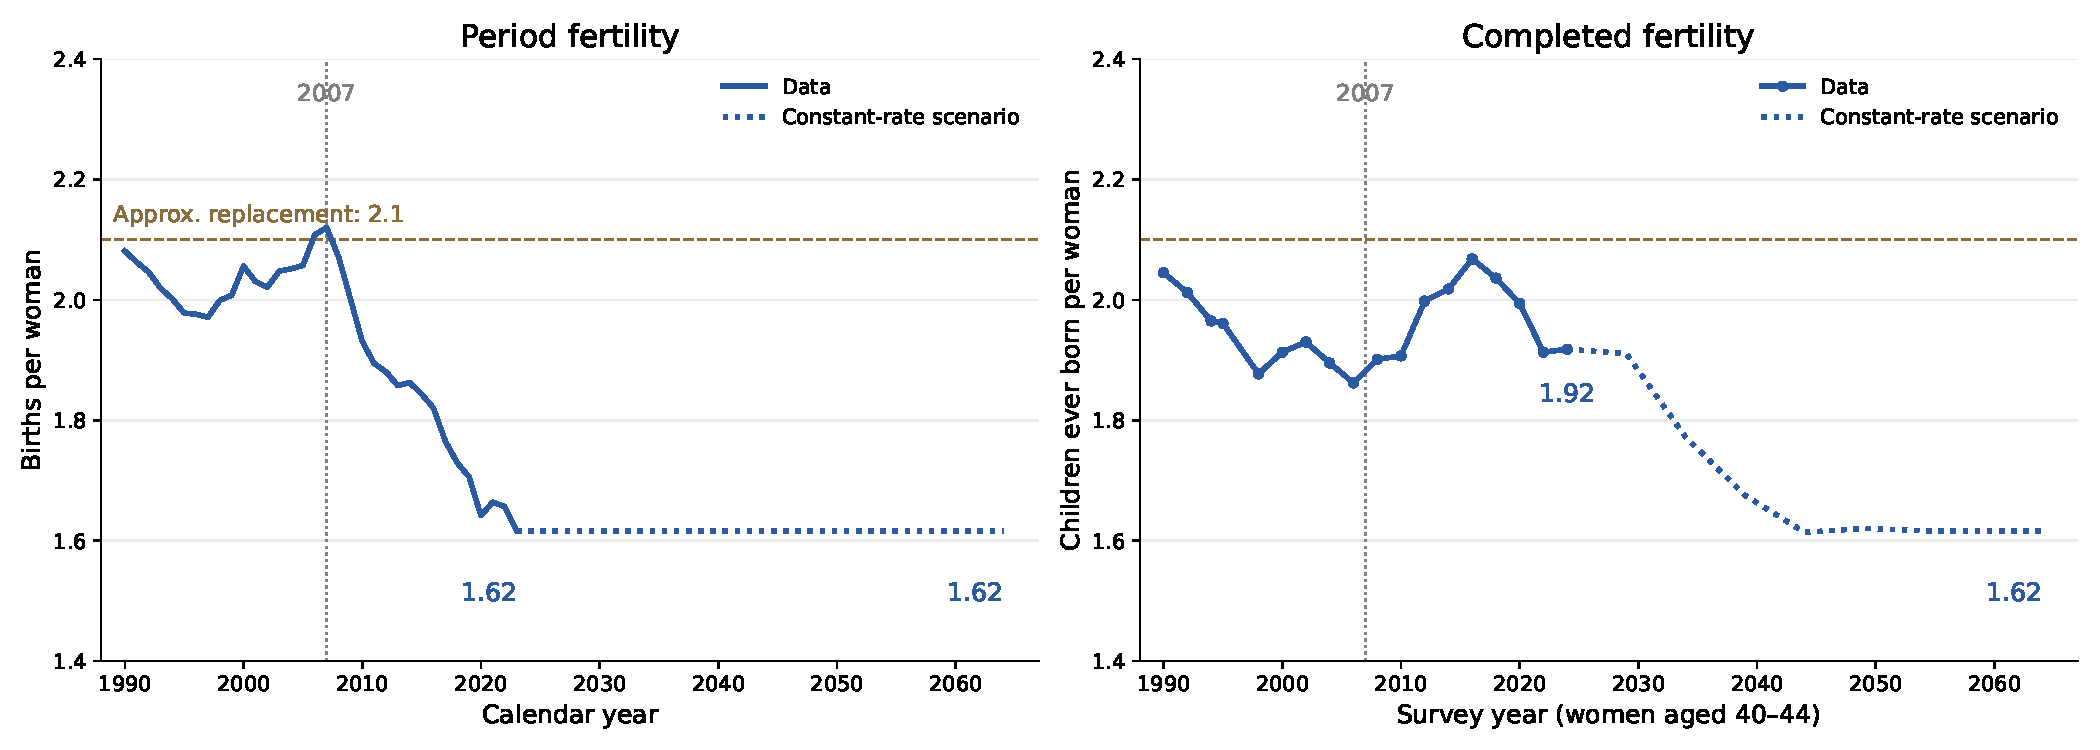
\includegraphics[width=\linewidth]{fertility_introduction_projection_1990}
\caption{Period and completed fertility in the United States}
\label{fig:quant-us-fertility}
\par\smallskip
\begin{minipage}{0.92\linewidth}
\footnotesize\textit{Notes:} Left: period total fertility rate, World
Development Indicators. Right: children ever born to women aged 40--44, CPS
Fertility Supplement. Dotted lines: a constant-rate scenario that holds period
fertility at its 2023 level; the completed-fertility continuation is rescaled
to end at that rate.
\end{minipage}
\end{figure}

The transition follows the logic of Section~\ref{sec:m-analysis}: fertility
falls first at about the inherited price, and the price falls as smaller
cohorts enter. I compare each policy experiment with the path the economy
follows from 2023 without it.

I divide the parameters of the 2007 economy into two groups. The first
group is assigned from external evidence or measured directly in the data.
The second is chosen so that the model matches a set of moments in the data.
Table~\ref{tab:quant-moments} reports the moments, and
Table~\ref{tab:quant-parameters} the parameters.

\subsection{Assigned parameters}
\label{sec:quant-data}
\label{sec:quant-period}

\begin{table}[!htbp]
\centering
\caption{Parameter values}
\label{tab:quant-parameters}
\small
\begin{tabularx}{\textwidth}{@{}l l X @{\hspace{1.5em}} l l X@{}}
\toprule
\multicolumn{3}{@{}l}{Assigned} & \multicolumn{3}{l}{Calibrated}\\
\midrule
$\sigma$ & 2 & risk aversion & $\beta_{\text{ann}}$ & 0.936 & annual discount factor \\
$(\omega,\nu)$ & 0.7, 0.7 & equivalence scale & $\psi_0$ & 0.177 & preference for children \\
$\alpha_0$ & 0.733 & consumption weight & $\gamma$ & 0.646 & curvature, benefit of children \\
$\lambda$ & $2/9$ & child departure, per period & $\xi$ & 0.295 & first-birth utility cost \\
$\pi_a$ & 0.98--0.50 & success of a birth attempt & $\kappa_1$ & 0.050 & first-birth taste scale \\
$\phi$ & 0.80 & financed share & $\kappa_C$ & 0.129 & later-birth taste scale \\
$\mu$ & 0.06 & selling cost & $h_P$ & 0.89 & space requirement (rooms) \\
$\delta_H$ & 0.014 & depreciation, annual & $\chi$ & 1.112 & owner service multiplier \\
$\tau^p$ & 0.0106 & property tax, annual & $\kappa_T$ & 0.013 & tenure taste scale \\
$r$ & 0.02 & real interest rate, annual & $\theta_0$ & 0.244 & bequest-motive scale \\
$\tau^w$ & 0.08 & payroll tax & $H_0$ & 6.776 & housing supply scale \\
% H0 = 5.7505 / 0.77069^0.63 = 6.776 with eta 0.63; 5.7505 = 2007 housing per household.
$\eta$ & 0.63 & housing-supply elasticity & & & \\
$\bar h^R$ & 6 & rental size cap (rooms) & & & \\
$\theta_1$ & 0.008 & bequest shifter & & & \\
$(\rho_z,\sigma_z)$ & 0.735, 0.484 & earnings, per four years & & & \\
\bottomrule
\end{tabularx}
\par\smallskip
\begin{minipage}{0.95\linewidth}
\footnotesize\textit{Notes:} Assigned parameters are set outside the
calibration (Section~\ref{sec:quant-data}); calibrated parameters are chosen
to match the moments of Table~\ref{tab:quant-moments}
(Section~\ref{sec:quant-identification}).
\end{minipage}
\end{table}

\paragraph{Demographics and timing.}
A period in the model lasts four years. Households enter at 18, retire at 66
and live at most through 85. Survival is certain before retirement and,
after it, follows the 2023 period life table of the Social Security
Administration. Births are possible through age 45. The success of an
attempt falls with age following the exponential schedule of
\citet{sommerFertilityChoiceLife2016}, from 0.98 at 18 to 0.90 at 30, 0.80
at 35 and 0.62 at 40.\problem{Source of the conception probabilities by age to be settled; not Sommer, not Leridon.} A child leaves home with probability $\lambda=2/9$ per
period, so children stay at home for 18 years on average.%
% pi_a = 1 - 0.02 exp(0.134 (a - 18)); 0.50 at 42. Leridon (2004) four-year
% conception 0.91 / 0.84 / 0.64 at 30 / 35 / 40 (docs/model/e5_target_review_20260724.md).
% Survival: 2023 SSA period life table, four-year ratios
% (docs/model/quantification_note_reaudit_and_study_guide_20260720.md).
\footnote{Stocks, such as wealth and house prices, are in annual units;
flows, such as income, consumption and rent, accrue over the four years.
Interest, discounting and depreciation compound over the period, so
$R_b=1.02^4$ and $\beta=\beta_{\text{ann}}^4$, and the property tax is four
times its annual rate. A data statistic for an age window weights each
four-year model cell by the share of the cell inside the window.}

\paragraph{Preferences.}
Flow utility \eqref{eq:m-utility} is
\begin{equation*}
 u(c,\hat h,n)=\frac{1}{1-\sigma}\left[\frac{c^{\alpha_0}\bigl(\hat h-\chi^{\1\{\text{own}\}}\,\bar h(n)\bigr)^{1-\alpha_0}}{e(n)}\right]^{1-\sigma}+\psi\,n^{1-\gamma},
 \qquad e(n)=\left(\frac{2+\omega n}{2}\right)^{\nu}.
\end{equation*}
I set the curvature to $\sigma=2$, a common choice in the literature. The equivalence scale
$e(n)$ is that of \citet{scholzSeshadriKhitatrakunSaving2006}, with
$\omega=\nu=0.7$: a couple with two children needs 1.45 times the
consumption, and the housing services above its requirement, of a childless
couple to reach the same utility. The consumption weight $\alpha_0=0.733$
is set to match the share of housing in the spending of childless renters in
the 2019--2023 CEX, 26.7\%. Indeed, a childless renter has no space
requirement and no owner multiplier, so its utility is Cobb--Douglas in
consumption and rented space, and it spends a share $1-\alpha_0$ of its
budget on rent.

\paragraph{Housing finance and taxes.}
The annual real interest rate is 2\%, and selling a home costs 6\% of its
value, as in \citet{greaneyDynamicUrbanEconomics2025}. Buyers can finance at
most $\phi=0.80$ of the price, the conventional limit above which a mortgage
requires private insurance, and there is no limit on payments relative to
income. I measure depreciation and the property tax at the national level,
with the method of \citet{greaneyDynamicUrbanEconomics2025}. Depreciation,
1.4\% a year, is the 2007 depreciation of owner-occupied residential
structures in the BEA fixed-asset accounts, divided by the value of the
housing stock, land included, in the Financial Accounts of the Federal
Reserve. The property tax, 1.06\% of value, is the ratio of aggregate
property taxes to the aggregate value of owner-occupied homes in the
2007--2011 ACS. Retirees receive a common pension equal to 23\% of mean
earnings, the ratio in the CPS ASEC, and the payroll tax that finances it is
8\%.
% Depreciation 0.01416143718381309, property tax 0.010598360773872594: CALIBRATION_STATUS
% (Sept 23 national housing-cost inputs; calibration_archive/context_refresh_20261002/
% CALIBRATION_STATUS.before.md l.4956). Pension/gross-earnings 0.2294460119, payroll tax
% 0.0802807096 (CALIBRATION_STATUS, Demography and closure).

\paragraph{Earnings.}
A household of age $a$ earns $e_az_t$, where
\begin{equation*}
 \log z_{t+1}=\rho_z\log z_t+\epsilon_{t+1},\qquad \epsilon_{t+1}\sim N(0,\sigma_z^2).
\end{equation*}
I estimate $\rho_z$ and $\sigma_z$ from the variance and first
autocovariance of log household earnings, averaged over non-overlapping
four-year spells and net of age and year effects, in the 1984--1997 PSID,
the last years in which the survey is annual. This gives $\rho_z=0.735$ and
$\sigma_z=0.484$, which I approximate with nine states. The age profile
$e_a$ is normalized to average one over working ages.\problem{Source of the
age profile $e_a$ to be confirmed.}
% output/model/native_financing_diagnostic_20260919/specification_followup/
% earnings_entry_battery_v1/single_process_external_estimate.json: gamma0 0.5085,
% gamma1 0.3735, held-out gamma2 0.2899 (model-implied 0.2744); rho = gamma1/gamma0,
% sigma_z = sqrt(gamma0 (1 - rho^2)).

\paragraph{Housing.}
Owners choose among homes of 2, 4, 6, 8 and 10 rooms, and renters any size
up to $\bar h^R=6$ rooms. The cap reflects the rental stock: in the 2023 AHS,
43\% of owner-occupied homes have seven or more rooms, against 7.5\% of
rented homes (Appendix~\ref{app:housing-stock}). The supply elasticity in
\eqref{eq:m-supply} is $\eta=0.63$, from the estimates of floor-space supply of
\citet{baum-snowMicrogeographyHousingSupply2024}.

\paragraph{Entry wealth.}
Households enter the economy with the wealth of young adults in the PSID: the
net worth of childless renters aged 18 to 24.
% POST-DEADLINE: check the entry sample years (current inputs pool PSID 1984-2019, N = 1,835,
% levels_rank, author-adopted Oct 5); he recalls a correction toward years around 2007.
Negative values are set to zero, since households
in the model cannot borrow without collateral.
% POST-DEADLINE: entry wealth is assigned to earnings states by rank (highest wealth to highest
% earnings), not matched to the data correlation; consider matching it as in Kaplan, Mitman and
% Violante (2020).

\paragraph{Bequests.}
In the bequest motive, $\theta_1$ determines how far bequests are a luxury
good. I set it to 1\% of median annual earnings in the model,
$\theta_1=0.008$, as in \citet{greaneyDynamicUrbanEconomics2025}.
% Entry law levels_rank (model/entry_wealth.py): PSID 1984-2019, N = 1,835, negative
% wealth censored at zero, one common scale, exact weighted-rank allocation to z.

\subsection{Calibrated parameters}
\label{sec:quant-identification}

I choose the remaining eleven parameters so that the 2007 steady state
matches the eleven moments in Table~\ref{tab:quant-moments}.%
\footnote{The parameters minimize a sum of squared gaps between model and
data moments, each divided by a tolerance for the moment
(Appendix~\ref{app:identification}).}
The parameters are chosen jointly, but some moments are more informative
about some parameters than others. I group them into five blocks and, for
each, describe the variation in the data that disciplines it and the
mechanism in the model through which it does.

As the model contains many contemporaneous interactions, there are several things to keep in mind to properly inform the differnt parameters. First, fertility and housing are determined together. In the
2007 steady state, the house price is the one at which completed fertility
equals replacement, so a parameter that lowers births also lowers the price,
and a lower price raises the space households occupy and how often they own.
I separate the two blocks with moments that respond to the price very
differently. How births are spread across women and over the life cycle,
measured by the shares of childless women and of mothers with one child and
by the mean age at first birth, barely moves with the price. Mean rooms and
ownership respond strongly to it. The housing moments therefore pin the
price, and the fertility moments pin the parameters that govern who has
children and when.
% 1% higher psi0: price +3.0%; childless +0.02%, one child +0.08%, mean age +0.01%;
% mean rooms -1.89%, ownership -1.32% (identification_newacct results.json, G*theta/m).
Second, households with children occupy more space than other households,
partly because a child requires space and partly because parents are older
and have higher earnings and savings. The change in rooms within households
at the first birth, relative to adults who never have a child, isolates the
space a child requires, $h_P$. The difference in ownership between recent
parents and other households measures how closely tenure follows these
needs, $\kappa_T$.
% POST-DEADLINE: locally h_P barely moves the event-study room response (elasticity -0.11;
% beta 7.73, psi0 1.78) and the ownership gap responds to h_P (1.18); revisit this pairing
% (identification_newacct results.json, G*theta/m).
Third, a change in when women
have children and a change in how many they have both move period fertility.
The distribution of completed family size at ages 40 to 44 measures how many
children women have, and the mean age at first birth measures when they
start.

\paragraph{Fertility.}
I choose the first-birth cost $\xi=0.295$ and the curvature $\gamma=0.646$
to match two shares among women aged 40 to 44 in the June Fertility
Supplement of the CPS, pooling 2004 and 2006: 19.8\% are childless, and
21.4\% of mothers have exactly one child. The cost is paid only at the first
birth, so a higher $\xi$ raises childlessness, and the same births then come
from fewer mothers with larger families. A higher $\gamma$ makes the benefit
of an additional child decline faster, so childlessness falls and more
mothers stop at one.

\paragraph{Timing of births.}
I include taste shocks in the fertility decision because, in the data,
otherwise similar households make different choices. First births are spread
over the whole fertile window, from the late teens to the early forties, and
women in the lowest third of family income have about as many children by
ages 40 to 44 as women in the top third. The shocks help explain this
idiosyncratic variation. The scale of the first-birth shocks,
$\kappa_1=0.050$, governs how much first births depart from the trade-off
between fecundity and earnings of Section~\ref{sec:m-analysis}. A larger
$\kappa_1$ spreads first births over the fertile window, so the mean age at
first birth, 26.0 years in the NCHS natality files for 2003--2006, rises,
and fewer women are mothers by age 25, 45.7\% in the CPS. I choose
$\kappa_1$ to match both. The estimate is small: first births follow the
economic trade-off closely, and the shocks mostly spread them across ages.
The scale for later births, $\kappa_C=0.129$, governs how readily mothers go
on to a second or third child. It is informed by the share of mothers with
exactly one child and by childlessness, since the option of further births
raises the value of becoming a parent.
% POST-DEADLINE: verify the CPS income-third fact (FACTS Oct 10: CEB 40-44 by family-income third,
% CPS June 2006/08, 1.98 / 1.81 / 1.82; model 1.50 / 1.97 / 2.31).

\paragraph{Preference for children.}
The preference $\psi_0$ is the taste for children in the 2007 steady state,
before the decline of Section~\ref{sec:quant-transition}. I choose it so that
completed fertility equals replacement, 2.1. This condition alone does not
pin $\psi_0$. Because the supply scale $H_0$ adjusts so that any price clears
the housing market, a higher $\psi_0$ together with a higher house price also
delivers 2.1 children. Housing demand identifies the difference: at a higher
price households occupy less space and own less often. The price, and with it
$\psi_0$, is therefore the one at which mean rooms are 5.73, as in the 2007
AHS, and ownership is 67.6\%. This gives $\psi_0=0.177$.
% psi_child is free in the loss; at each trial value the price is the root of
% adjusted_births/(2.1*entry)-1 (equilibrium.py) and H0 is implied at population one.
% 1% higher psi0: price +3.0%, mean rooms -1.9% (identification_newacct moments).

\paragraph{Housing and tenure.}
I choose the owner multiplier $\chi=1.112$ to match ownership among heads
aged 30 to 55 in the 2005--2006 ACS, 67.6\%.%
\footnote{Both ownership samples exclude mobile homes, boats and vans (ACS
structure codes 3 to 10), which have no counterpart in the model.}
An owner obtains $\chi$ times the services of the same home, so a higher
$\chi$ raises the value of owning relative to renting.

The space requirement $h_P=0.89$ rooms is disciplined by the change in
housing within households at the first birth. Recall from
Section~\ref{sec:emp-first-birth} that future parents in the PSID live in
4.71 rooms two to three years before the first birth, and three to four years
after it occupy 1.44 more rooms, relative to the change among adults who
never have a child. I run the same regression on households in the model.
% Production target: output/model/first_birth_rooms_event_20261010/
% measurement_bridge/proposed_measurement_contract.json and original/rooms_coefficients.csv;
% adopted in output/model/production/2007/PROMOTION_RECEIPT_20261011_7p917.md.
% Common-support A2h target 1.439960832044094; model 1.4755 at the new point
% (identification_newacct moments/center.json, birth_dated +3/+4).
The requirement is the space a household must add once it has a child, and
this jump is the most direct measure of it in the data.

The tenure taste scale $\kappa_T=0.013$ is disciplined by the difference in
ownership between recent parents and other households. In the ACS, heads
whose oldest child is under four own at a rate
12.8 percentage points higher than heads with no children at home. In the
model, homes larger than $\bar h^R$ rooms are only for sale, so the space
requirement pushes parents into ownership. A smaller $\kappa_T$ makes tenure
follow these needs more closely and widens the gap.
% POST-DEADLINE: see the note on the h_P / kappa_T pairing above.

\paragraph{Wealth and bequests.}
I choose the discount factor $\beta=0.936$ (annual) to match aggregate net
worth of 4.46 times aggregate annual gross labor earnings in the PSID.%
\footnote{Net worth of heads aged 18 to 85, excluding business and farm
equity and other real estate; gross labor earnings of heads aged 18 to 65.}
More patient households save more, so wealth accumulation responds
directly to $\beta$. Savings also decide when a household can pay for the space a
child requires, so $\beta$ moves fertility and housing as well. The bequest
scale $\theta_0=0.244$ governs how much wealth households keep for their
heirs in old age. I choose it to match the annual flow of estates to
children in the 2007 SCF, 0.73\% of aggregate net worth.

As Table~\ref{tab:quant-moments} shows, the model matches
these targets closely. Childlessness is 20.1\% in the model and 19.8\% in
the data, ownership 66.9\% and 67.6\%, the recent-parent ownership gap 12.5
and 12.8 percentage points, and wealth 4.35 and 4.46 times annual earnings.

\begin{table}[!htbp]
\centering
\caption{Moments used in the calibration}
\label{tab:quant-moments}
\small
\begin{tabularx}{0.8\textwidth}{@{}X r r@{}}
\toprule
Moment & Data & Model \\
\midrule
Completed fertility & 2.10 & 2.10 \\
Childless, women 40--44 (\%) & 19.8 & 20.1 \\
Exactly one child, mothers 40--44 (\%) & 21.4 & 21.7 \\
Mean age at first birth (years) & 25.98 & 25.97 \\
Mothers by age 25 (\%) & 45.7 & 45.5 \\
\addlinespace
Mean occupied rooms & 5.73 & 5.75 \\
Ownership, heads 30--55 (\%) & 67.6 & 66.9 \\
Recent-parent ownership gap & 0.128 & 0.125 \\
First-birth room response & 1.440 & 1.475 \\
\addlinespace
Wealth / annual gross earnings & 4.46 & 4.35 \\
Annual bequests / wealth (\%) & 0.73 & 0.73 \\
\bottomrule
\end{tabularx}
\par\smallskip
\begin{minipage}{0.95\linewidth}
\footnotesize\textit{Notes:} Fertility: CPS June Fertility
Supplement 2004 and 2006, women 40--44, and mothers by 25; NCHS natality 2003--2006 for the mean age at first birth;
completed fertility is a normalization. Housing: AHS 2007 for rooms; ACS
2005--2006 for ownership and the gap between heads whose oldest child is
under four and heads without children; PSID event study for the room
response, measured in the model with the same design on simulated
households. Wealth: PSID 2005 and 2007; bequests: SCF 2007. Owners choose
among homes of 2, 4, 6, 8 and 10 rooms. The 2007 house price is 0.771.
% POST-DEADLINE: mothers by 25 replaces children ever born by 25 as a target (his word Oct 25);
% the parameters were estimated with CEB-by-25 (loss 7.42, CEB25 6.41). Re-estimate and check identification.
\end{minipage}
\end{table}




\subsection{The fertility decline, 2007--2023}
\label{sec:quant-transition}

Starting from the 2007 steady state, I hold all estimated parameters fixed
and let the preference for children decline permanently from its 2007 level
$\psi_0$ toward a lower level $\psi'$,
\begin{equation}
\psi_t=\psi'+(\psi_0-\psi')\,\rho^{\,\tau},
\label{eq:psi-decay}
\end{equation}
where $\tau$ counts four-year periods since 2007. Households learn the whole
path in 2007 and have perfect foresight about it and about prices. The house
price, the pension and the rebate clear their markets at every date
(Appendix~\ref{app:algorithms}). I set $\rho=0.35$ and choose
$\psi'=0.148$ to match period fertility in 2020--2023, 1.646
(Figure~\ref{fig:quant-transition-fit}).%
\footnote{A model period is dated by its first year and compared with the
average period fertility of the four following calendar years: the period
dated 2019 with 2020--2023.}
The decline in $\psi_t$ summarizes changes in the incentives to have
children that the model does not otherwise capture.%
\footnote{See \citet{kearneyPuzzleFallingUS2022} and
\citet{doepkeEconomicsFertilityNew2023} for reviews of the recent decline in
fertility and its possible causes.}
From the period dated 2023 on, period fertility is 1.63 and
rises slowly, to 1.73 by 2063.

\begin{figure}[!htbp]
\centering
\includegraphics[width=0.7\linewidth]{../../output/model/production_runs/2026-10-24_transition_fi/fertility_fit_fi_2007_2063_single.pdf}
\caption{Period fertility, model and data, 2007--2063}
\label{fig:quant-transition-fit}
\par\smallskip
\begin{minipage}{0.92\linewidth}
\footnotesize\textit{Notes:} Model: births per woman in each four-year
period of the transition from the 2007 steady state. Data: annual period fertility and its
four-year averages.
\end{minipage}
\end{figure}

Figure~\ref{fig:quant-full-transition} shows the whole transition. Period
fertility returns to replacement slowly: it is 2.09 by 2203, and by 2403 the
economy is at its new steady state, with the number of households at 49\%,
total housing at 67\% and the house price at 53\% of their 2007 levels.
As the population shrinks, the house price falls: it is 3.6\% below its
2007 level in 2023 and 19.3\% below in 2063. The rent does not follow
the price down at first. Along a transition, rent equals the user cost net of
the expected capital gain, so a price that is expected to keep falling raises
the rent: in 2023 the rent per room is 2.0\% above its 2007 level.

To illustrate the role of the housing stock in determining fertility in the
model, the dashed lines in Figure~\ref{fig:quant-full-transition} show the
same transition with the total housing stock $H$ held at its 2023 level from
2023 on. With a fixed stock, the price falls much further, to 47\% of its
2007 level around 2111. At that price fertility overshoots replacement,
reaching 2.18 around 2119, and the additional children fill the fixed stock a
generation later. As they do, the price recovers and fertility returns to
replacement. In the long run the price is the same as in the baseline, 53\%
of its 2007 level, because fertility at replacement pins it; the stock
determines only how many households live at that price, 71\% of the 2007
level instead of 49\%. This suggests a potential role for housing supply in
speeding up the recovery of fertility, which I explore in
Section~\ref{sec:policy}.
% Oct 25: target windows read from FIN063fi_fw.json decay block (target_2011 1.861 = WDI mean 2012-15,
% target_2019 1.64575 = 2020-23) and the fit figure script (data averages over t+1..t+4).
% [MODEL, Oct 24] FIN063fi_fw.json (free entry, eta 0.63, rho 0.35, psi_inf 0.148414,
% psi_2007 0.177467; converged, 100 periods, terminal steady state reached by 2403):
% output/model/experiments/housing_supply/20261022_fi_all_arms/history/. TFR 2011 1.7394,
% 2019 1.6458, 2023 1.6313, 2063 1.7319, 2203 2.0891, 2403 2.1001; price/0.770686 2023 0.964,
% 2063 0.807, 2403 0.529; stock/5.752224 2023 0.977, 2063 0.874, 2403 0.669; households 2403
% 0.488; construction H_t-(1-delta)H_{t-1} between 0.19 and 0.30 at every date; rent 2023
% 0.13350 vs 0.13085 in the 2007 steady state. Figures:
% production_runs/2026-10-24_transition_fi/plot_transition_fi_eta063.py.

\begin{figure}[!htbp]
\centering
\includegraphics[width=0.85\linewidth]{../../output/model/production_runs/2026-10-24_transition_fi/full_transition_four_panel_fi_eta063_fixedstock.pdf}
\caption{The full transition, 2007--2403}
\label{fig:quant-full-transition}
\par\smallskip
\begin{minipage}{0.92\linewidth}
\footnotesize\textit{Notes:} Period fertility, number of household heads,
total housing and the house price along the transition, with the initial
steady state normalized to 100. Dashed: the same transition
with the housing stock held at its 2023 level from 2023 on.
\end{minipage}
\end{figure}


\subsection{Testing the model}
\label{sec:quant-fit}

I conclude by comparing the model with some moments that the calibration
does not target, reported in Table~\ref{tab:quant-untargeted}. The first is
how many children mothers have beyond the first. This matters because the
space requirement does not rise with the number of children, so later births
test the other costs and benefits of children in the model. The calibration
targets the share of women with no children and the share of mothers with one
child, but not how the remaining mothers split between two children and three
or more. The model matches this split: 32.2\% of women aged 40 to 44 have two
children and 30.4\% have three or more, against 34.4\% and 28.6\% in the CPS.
The second is the timing of first births, which matters because the central
trade-off in the model is one of timing, between fecundity that falls with
age and earnings and savings that rise with it. The model matches the share
of first births at 30 or later, 24.2\% against 24.9\% in the natality files.
The third is the dispersion of wealth among the old, which reflects how much
households save: the ratio of the 90th percentile to the median of wealth
relative to income at ages 76 to 84 is 3.27 in the model and 3.52 in the
PSID. The model fits two housing moments less well. Children are linked to
housing in the model through the space they require and the ownership of
large homes. Households with three or more children occupy 0.57 more rooms
than those with one or two, against 0.39 in the data, and ownership rises
around the first birth by 14 percentage points, against 26.
% [MODEL] family size: kappa_identification/stage3/runs/center/.../observers.json uniform_birth_time
% parity_shares_40_44 (20.0/17.3/32.2/30.4); [DATA] 2026-10-25_data_pictures/cps_family_size_40_44.json
% (CPS June 2004/06, n = 10,872: 19.8/17.1/34.4/28.6).

\begin{table}[!htbp]
\centering
\caption{Moments not targeted, 2007}
\label{tab:quant-untargeted}
\small
\begin{tabularx}{\textwidth}{@{}X l r r@{}}
\toprule
Moment & Source & Data & Model \\
\midrule
First births at age 30+ (\%) & NCHS 2003--2006 & 24.9 & 24.2 \\
Rooms: 3+ versus 1--2 resident children & ACS 2005--2006 & 0.385 & 0.574 \\
First-birth ownership response & PSID event study & 0.261 & 0.141 \\
Wealth/income p90 / median, ages 76--84 & PSID & 3.52 & 3.27 \\
\bottomrule
\end{tabularx}
\par\smallskip
\begin{minipage}{0.95\linewidth}
\footnotesize\textit{Notes:} This table reports moments that do not enter
the loss \eqref{eq:q-loss}. The ownership response is the event-study
coefficient of Section~\ref{sec:empirical-evidence} on the model's
observation support, measured on simulated households with the same design.
% [MODEL] moments/center.json target_fit validation rows: share30 0.2421,
% family_rooms 0.5740, old_dispersion 3.2730 (7.9: 3.4656, same row); ownership
% event birth_dated Wp3 0.1410.
\end{minipage}
\end{table}

Figure~\ref{fig:quant-lifecycle-2007} compares life-cycle profiles of
ownership, rooms and first births by age with the data. The calibration
targets only averages, ownership among heads aged 30 to 55, mean rooms and
the mean age at first birth, so the shape of these profiles is not
targeted. The model reproduces the rise of ownership with
age, and between 34 and 49 the two profiles are within four percentage
points. It also reproduces the hump in housing size: rooms rise until the
forties and then decline, although the model profile is steeper. First
births by age of the mother follow the data closely. Young households own
too often in the model, 34\% at 18--21 and 44\% at 22--25, against 12\% and
24\% in the data, and older households keep their homes, since the model has
no health or long-term-care risk that would lead them to sell.
% [MODEL] output/model/calibration/2026-10-21_lifecycle_newacct/lifecycle_2007_newacct.json;
% [DATA] output/model/production/2007/plotted_long.csv (ACS 2005/06, rooms capped at 9;
% NCHS 2005-07 first births).

\begin{figure}[!htbp]
\centering
\includegraphics[width=\linewidth]{../../output/model/calibration/2026-10-21_lifecycle_newacct/lifecycle_2007_newacct.pdf}
\caption{Life-cycle profiles in 2007, model and data}
\label{fig:quant-lifecycle-2007}
\par\smallskip
\begin{minipage}{0.92\linewidth}
\footnotesize\textit{Notes:} Homeownership and rooms by age of the household
head, and the distribution of first births by age of the mother. Model: 2007
steady state. Data: ownership and rooms (at most nine) from the 2005--2006
ACS; first births by four-year age group from the NCHS natality files for
2005--2007.
\end{minipage}
\end{figure}

Appendix~\ref{sec:quant-2023} compares the 2023 economy, the starting point
of the policy experiments, with the 2023 data. None of these moments is
targeted by the transition. The model reproduces the direction of the shift
in the timing of births: from 2007 to 2023 the share of women who are mothers
by 25 falls by 13 percentage points in the model and by 18 in the data, in
line with the fall in birth rates at younger ages documented by
\citet{kearneyPuzzleFallingUS2022}. It also matches the share of mothers
with one child, 22.2\% in both, and mean rooms, 5.51 against 5.58. Two
misses are informative about what a decline in preferences alone leaves out.
First, in the model the decline works on every cohort alive, so childlessness
among women aged 40 to 44 rises to 28.7\%, while in the data it barely moved,
from 19.8\% to 18.8\%. Second, fewer births lower the demand for family
space, so the model's house price falls by 3.6\%, while in the data the real
house price rose by 15.6\%.%
\footnote{Two features of the model limit its account of house prices over
this period. First, the model starts from a stationary population, so it
misses the momentum of the actual age distribution of 2007, which kept
household formation growing after 2007. Second, the model has no aggregate shocks to credit or income, so it
does not capture the boom and bust in house prices around 2007. It is built
to study medium- and long-run trends.}
The transition shows how housing responds to a decline in fertility; it does
not attribute the decline to housing.
\problem{Testing the model: possible additions tomorrow, such as a 2023
figure or other untargeted fits that work well.}
% [MODEL 2023] moments_2023_fi.csv free_entry_eta0.63; mothers by 25 32.2 (validation json), 2007 45.5.
% [DATA] Case-Shiller CSUSHPINSA / CPIAUCSL 2023/2007 = 1.156 (historical_supply_comparison.csv).

% Section 5, Testing the model (split from the quantification section, Oct 25 2026).
% 2007 fit: output/model/calibration/2026-10-19_identification_newacct/ (moments/center.json) and
% output/model/calibration/2026-10-21_lifecycle_newacct/. 2023: experiments/housing_supply/20261021_free_entry/
% moments_2023_fi/ (free_entry_eta0.63 column; replay of the converged FIN063fi_fw history).

\section{Testing the model}
\label{sec:quant-fit}

In this section I compare the model with features of the data that the
calibration does not target. I focus on the margins that matter for the
policy experiments of Section~\ref{sec:policy}: how many children women have
and when, how households change their housing around a birth, and how
ownership and housing evolve over the life cycle.
Table~\ref{tab:quant-untargeted} reports the untargeted moments, and
Figures~\ref{fig:quant-family-size} to~\ref{fig:quant-event-scatter} compare
the full distributions and profiles. Appendix~\ref{sec:quant-2023} compares
the 2023 economy, the starting point of the policy experiments, with the
2023 data.

\begin{table}[t]
\centering
\caption{Moments not targeted, 2007}
\label{tab:quant-untargeted}
\small
\begin{tabularx}{\textwidth}{@{}X l r r@{}}
\toprule
Moment & Source & Data & Model \\
\midrule
First births at age 30+ (\%) & NCHS 2003--2006 & 24.9 & 24.2 \\
Rooms: 3+ versus 1--2 resident children & ACS 2005--2006 & 0.385 & 0.574 \\
First-birth ownership response & PSID event study & 0.261 & 0.141 \\
Wealth/income p90 / median, ages 76--84 & PSID & 3.52 & 3.27 \\
\bottomrule
\end{tabularx}
\par\smallskip
\begin{minipage}{0.95\linewidth}
\footnotesize\textit{Notes:} This table reports moments that do not enter
the loss \eqref{eq:q-loss}. The ownership response is the event-study
coefficient of Section~\ref{sec:empirical-evidence} on the model's
observation support, measured on simulated households with the same design.
% [MODEL] moments/center.json target_fit validation rows: share30 0.2421,
% family_rooms 0.5740, old_dispersion 3.2730 (7.9: 3.4656, same row); ownership
% event birth_dated Wp3 0.1410.
\end{minipage}
\end{table}

\subsection{Fertility}
The model reproduces the distribution of completed family size
(Figure~\ref{fig:quant-family-size}). The calibration targets the share of
women with no children and the share of mothers with one child. It does not
target how the remaining mothers split between two children and three or
more. In the model, 32.2\% of women aged 40 to 44 have two children and
30.4\% have three or more, against 34.4\% and 28.6\% in the CPS. The timing
of first births is also close to the data: 24.2\% of first births occur at
30 or later, against 24.9\% in the natality files. The right panel of
Figure~\ref{fig:quant-lifecycle-2007} shows the whole distribution. The
model places fewer first births between 26 and 33, 28.5\% against 33.6\%,
and more at 18 to 21.
% [MODEL] family size: kappa_identification/stage3/runs/center/.../observers.json uniform_birth_time
% parity_shares_40_44 (20.0/17.3/32.2/30.4); [DATA] 2026-10-25_data_pictures/cps_family_size_40_44.json
% (CPS June 2004/06, n = 10,872: 19.8/17.1/34.4/28.6).

\begin{figure}[tbp]
\centering
\includegraphics[width=0.55\linewidth]{../../output/model/calibration/2026-10-25_data_pictures/family_size_2007.pdf}
\caption{Completed family size, model and data}
\label{fig:quant-family-size}
\par\smallskip
\begin{minipage}{0.92\linewidth}
\footnotesize\textit{Notes:} Share of women aged 40 to 44 by number of
children ever born. Model: 2007 steady state. Data: June Fertility Supplement
of the CPS, 2004 and 2006 pooled.
\end{minipage}
\end{figure}

\begin{figure}[tbp]
\centering
\includegraphics[width=\linewidth]{../../output/model/calibration/2026-10-21_lifecycle_newacct/lifecycle_2007_newacct.pdf}
\caption{Life-cycle profiles in 2007, model and data}
\label{fig:quant-lifecycle-2007}
\par\smallskip
\begin{minipage}{0.92\linewidth}
\footnotesize\textit{Notes:} Homeownership and rooms by age of the household
head, and the distribution of first births by age of the mother. Model: 2007
steady state. Data: ownership and rooms (at most nine) from the 2005--2006
ACS; first births by four-year age group from the NCHS natality files for
2005--2007.
\end{minipage}
\end{figure}

\subsection{Housing around the first birth}
Figure~\ref{fig:quant-event-scatter} compares the change in rooms and in
ownership around the first birth in the model and in the PSID, window by
window. The calibration targets only the change in rooms three to four years
after the birth. The rest of the room response after the birth is close to
the data for about eight years: in the window of the birth, households add
0.78 rooms in the model and 0.62 in the data. Two differences stand out.
First, model households already add rooms in the years before the birth,
while in the data rooms are flat before it. Second, ownership rises around
the first birth by 14 percentage points in the model, against 26 in the
data.
% [MODEL] center.json first_birth_event_path, birth_dated (omitted -3/-2): <=-8 -0.65,
% -7/-6 -0.53, -5/-4 -0.20, -1/0 0.78, +1/+2 1.51, +3/+4 1.48, >=11 0.65; ownership_event Wp3 0.141.
% [DATA] rooms_coefficients.csv (A2h, common support), ownership A2h_own: Wp3 0.261.

\begin{figure}[tbp]
\centering
\includegraphics[width=0.85\linewidth]{../../output/model/calibration/2026-10-25_data_pictures/untargeted_event_scatter.pdf}
\caption{Housing around the first birth, model and data}
\label{fig:quant-event-scatter}
\par\smallskip
\begin{minipage}{0.92\linewidth}
\footnotesize\textit{Notes:} Each point is a two-year window around the
first birth, relative to the window two to three years before it. Data: the
PSID event study of Section~\ref{sec:empirical-evidence}. Model: the same
regression on simulated households in the 2007 steady state. The hollow
marker is the targeted room response.
\end{minipage}
\end{figure}

\subsection{Life-cycle profiles}
Figure~\ref{fig:quant-lifecycle-2007} compares ownership and rooms by age of
the head with the 2005--2006 ACS. The model reproduces the rise of
ownership with age, and between 34 and 49 the two profiles are within four
percentage points. It also reproduces the hump in housing size: rooms rise
until the forties and then decline, although the model profile is steeper.
Young households own too often in the model, 34\% at 18--21 and 44\% at
22--25, against 12\% and 24\% in the data. Older households keep their homes
in the model, since it has no health or long-term-care risk that would lead
them to sell.
% [MODEL] output/model/calibration/2026-10-21_lifecycle_newacct/lifecycle_2007_newacct.json;
% [DATA] output/model/production/2007/plotted_long.csv (ACS 2005/06, rooms capped at 9;
% NCHS 2005-07 first births).

\subsection{Wealth}
The model accounts for the dispersion of wealth among the old: the ratio of
the 90th percentile to the median of wealth relative to income at ages 76 to
84 is 3.27, against 3.52 in the PSID.

% Section 5, rewrite of October 21, 2026. Stationary solves at the estimated
% point (loss 7.4186) and the 2007 price 0.7707, rebate balanced in each solve.
% Figures and values: output/model/experiments/first_child_cost/20261021/
% (fig_s5_*.pdf, s5_values.json, scripts/s5_figs.py).
\newcommand{\FCC}{../../output/model/experiments/first_child_cost/20261021}

\section{Household Choices in the Calibrated Model}
\label{sec:results}

This section describes how households in the calibrated model respond to parenthood, and how earnings risk shapes the decision to have one. First, I show how having children changes housing, consumption and
tenure. The child's space trades off with consumption, so the cost
weighs most on households with little wealth or low earnings. Second, I illustrate how
 lowering the standard deviation of earnings shocks by about a quarter,
holding the house price at its 2007 level, raises completed fertility by 12\%.

\subsection{Choices at the first birth}
\label{sec:results-policy-functions}

Figure~\ref{fig:results-policy} compares the choices of the same household in
the period in which it has no child and in the period in which a first child
is born. The household is a renter aged 26 to 29 with median earnings, and
the figure varies its liquid wealth. Without savings, a first child pushes the
space the household rents close to the rental cap and lowers the probability
of owning from 42\% to 24\%. The child needs space when the household can
least afford a down payment, so it rents and pays for the space out of
consumption. With more than about two years of earnings in liquid wealth, the
child instead raises the probability of owning, and the household buys a
larger home.

Panel (d) shows the value of trying for a child, $V^F_{t,A}-V^F_{t,0}$. It is
negative without savings, turns positive at about five months of earnings,
and rises steeply at low wealth before flattening. Wealth therefore matters
for the decision to have a first child mostly among households with little
of it.

\begin{figure}[!tb]
\centering
\includegraphics[width=0.72\linewidth]{\FCC/fig_s5_choices.pdf}
\caption{Choices with and without a first child}
\label{fig:results-policy}
\par\smallskip
\begin{minipage}{0.92\linewidth}
\footnotesize\textit{Notes:} Renter aged 26--29 with median earnings
($z=0.78$), 2007 stationary equilibrium. Liquid wealth in units of mean annual earnings.
Rooms and consumption are averages over tenure choices.
\end{minipage}
\end{figure}

\subsection{Choices across earnings}
\label{sec:results-cost}

Figure~\ref{fig:results-cost} repeats the comparison across earnings states,
for renters aged 26 to 29 without savings. A first child adds about two thirds
of a room at earnings up to the median, and about half a room at high earnings,
where most of these households buy a home even without a child. Consumption falls
by 21\% at the lowest state and by 2\% at the median state. At high earnings
it rises, because the equivalence scale raises the household's needs and
these households can afford to meet them. As Section~\ref{sec:m-analysis} shows, the space requirement alone
costs about $r_th_P$ in every period the child is at home, whether the
household rents or owns. At the 2007 price, this is 2.9\% of mean annual
earnings each year. The cost of a child's space is therefore a recurring
expense, and it weighs most on households with low earnings.

\begin{figure}[!b]
\centering
\includegraphics[width=\linewidth]{\FCC/fig_s5_cost_by_earnings_all9.pdf}
\caption{Choices with and without a first child, by earnings}
\label{fig:results-cost}
\par\smallskip
\begin{minipage}{0.92\linewidth}
\footnotesize\textit{Notes:} Renters aged 26--29 without savings, 2007
stationary equilibrium, by earnings state $z$. Rooms and consumption are
averages over tenure choices. The dashed line marks the rental cap $\bar h^R$.
\end{minipage}
\end{figure}

\subsection{Earnings risk}
\label{sec:results-risk}

Section~\ref{sec:m-analysis} showed that earnings risk raises the expected
cost of a child, since that cost falls with earnings at a decreasing rate. To
measure this force, I lower the standard deviation of the four-year earnings
shock by about a quarter, from 0.48 to 0.35, rescale the earnings states to keep mean earnings
unchanged, and solve the model at the 2007 price. Lower risk raises completed
fertility by 12\%, from 2.10 to 2.36.\footnote{Without the rescaling, the same
change raises mean earnings by 4.9\%, and completed fertility rises by 16\%.}
Figure~\ref{fig:results-risk-floor} below reports the effect over a range of
values of earnings risk.

Figure~\ref{fig:results-risk} shows where the additional births come from.
In the baseline, the model matches the distribution of children ever born
among women in their early forties. Lower risk shifts households out of
childlessness and toward larger families: the share without children falls
from 20\% to 12\%, and the shares with two and with three or more rise.

\begin{figure}[!tb]
\centering
\includegraphics[width=0.6\linewidth]{\FCC/fig_s5_risk_children.pdf}
\caption{Earnings risk and children ever born}
\label{fig:results-risk}
\par\smallskip
\begin{minipage}{0.92\linewidth}
\footnotesize\textit{Notes:} Shares with 0, 1, 2, and 3 or more children
ever born. Data: CPS June Fertility Supplement, 2006 and 2008, women aged
40--44. Model: households at about age 42, 2007 stationary equilibrium, at
the estimated earnings risk ($\sigma_z=0.48$, baseline) and at lower risk
($\sigma_z=0.35$, earnings states rescaled to keep mean earnings unchanged),
same price.
\end{minipage}
\end{figure}

Earnings risk weighs more when a child requires more space.
Figure~\ref{fig:results-risk-floor} solves the model at the 2007 price for
different values of the space a child requires, $h_P$, and of the standard
deviation of earnings shocks. Lowering risk to 0.35 raises completed
fertility by 10\% when a child requires half a room, and by 17\% when it
requires 1.6 rooms. The child's space must be paid in every period the child
is at home, including after a bad earnings draw, when consumption is most
valuable. The more space a child requires, the more these periods cost, and
the more a household gains from lower risk.

\begin{figure}[H]
\centering
\includegraphics[width=0.65\linewidth]{\FCC/fig_s5_risk_floor25.pdf}
\caption{Earnings risk and the space a child requires}
\label{fig:results-risk-floor}
\par\smallskip
\begin{minipage}{0.92\linewidth}
\footnotesize\textit{Notes:} Completed fertility, \% change from the
baseline (marked), 2007 stationary equilibrium, same price, on a grid of 25
values of each parameter. Vertical axis: standard deviation of the four-year
earnings shock, with earnings states rescaled to keep mean earnings
unchanged. Horizontal axis: space a child requires, $h_P$, in rooms.
\end{minipage}
\end{figure}

% Section 6, rewrite of October 22, 2026 (his words 04:12Z): closer to the slides. Two exercises compared, matched supply and
% mortgage credit (quantum and tempo); then who uses the credit (the decomposition); then credit for parents; then cash,
% insurance and a rebated property tax. The +10% supply arm is dropped from the main text. One elasticity (0.63) in the main
% text; eta 1.5 and the slow stock in Appendix D. Main text = free entry (his decision Oct 21 22:36Z).
% NUMBERS ARE PLACEHOLDERS (his word 03:52Z): the slides' runs, OLD SETUP = instant supply eta 0.63, old accounting, 7.9
% calibration, constant-decay state: 20261021_paper_results/p6_values_oldsetup.json and the three fig_p6_*_oldsetup_eta063.pdf
% (p6_figs_oldsetup.py, from 20261017_accounting/transitions/data/prod_*); 2023 tenure of ages 22-29:
% transitions_2023/decay_ship_20261014/tenure_size_22_29_2023_decay.json. \oldv marks every placeholder.
% The 2007 stationary credit figure (\FCC) is at the current calibration. Earlier versions in git.
% Oct 22 15:30Z: FREE-ENTRY numbers filled where the arm has converged (credit, parents, cash, insurance; base TFR):
% 20261021_paper_results/p6_values_fi.json and fig_p6_{paths,transfers}_fi_eta063.pdf (p6_figs_fi.py, from
% 20261017_accounting/transitions/data_fi_torch/P063fi_*.json = Torch pol_063fi/out/runs/*/result.json). Credit is UNDER CHECK
% (1.35% vs about 1.9% on the slides). Still \oldv (red, slides' runs): matched supply, property tax, the 22-29 tenure split, and
% the quantum-tempo figure (needs matched supply).
\providecommand{\pend}{\textcolor{red}{[pending]}}
\providecommand{\oldv}[1]{\textcolor{red}{#1}}
\providecommand{\chk}{\textcolor{red}{$^{\ddagger}$}}
\newcommand{\PRF}{../../output/model/experiments/housing_supply/20261021_paper_results}

\section{Counterfactuals}
\label{sec:policy}

In this section, I use the calibrated model to study counterfactual changes to
the 2023 economy and unpack the interaction between family space and
fertility. First, I show that relaxing credit and expanding the housing
supply raise births by the same amount on impact but have different effects
over time, with housing supply having a stronger long-run effect. Second, I show that the main reason credit moves births earlier, but doesn't have as strong of a permanent effect, is  because young
households use it to buy the small homes they would otherwise rent. Intuitively, credit lowers
the down payment, not the cost of the space a child needs. Third, I show that
credit tied to children, which does lower that cost, raises the completed
fertility of the 2023 cohort by 4.9\%, and I compare these changes with a
property tax.


\subsection{Credit relaxation and housing supply}
\label{sec:policy-design}

I compare two changes that intervene in the housing market. The first relaxes
credit: the loan-to-value limit $\phi$ rises from 80\% to 100\%, so buyers no
longer need a down payment. As Section~\ref{sec:m-analysis} shows, credit
raises the probability of trying for a child only if it is worth more to a
household with the additional child than without it \eqref{eq:m-credit}. Importantly, it
can raise fertility when the down payment stands between a household and the
home its family needs. The quantification is hence an important tool to assess whether there is a significant mass of agents that are giving up on having kids due to their inability of affording a `family home' with many rooms. The second change expands the housing supply: the scale of
the supply curve \eqref{eq:m-supply}, $H_0$, rises by 4.35\%, so that at any price the stock
is 4.35\% larger. I choose this size so that births in 2023 rise by as
much as under the credit policy. Credit lowers the down payment needed to buy a home.
Supply lowers the cost of housing, both the price and rents. With the same
effect on impact, the comparison shows which of the two costs matters for
fertility.

Both experiments start from the 2023 state of the transition in
Section~\ref{sec:quant-transition}. In 2023 the change is announced unexpectedly and
understood to be permanent by agents. I compare each experiment with the path the economy follows from
the same state without the change. The preference for children follows the
same path with and without the change. Appendix~\ref{app:policy-robust} repeats the
experiments with a more elastic supply and with a slowly adjusting stock.

I report births in the four-year periods starting in 2023 and 2063 and in the
long run, when the economy reaches its new stationary equilibrium, and the
completed fertility of the cohort aged 18 to 21 in 2023: the children ever
born to these households over their lives. All are relative to the no-policy
path. Table~\ref{tab:policy-main} summarizes the results; it also reports
credit for parents, which Section~\ref{sec:policy-parents} describes.

\begin{table}[H]
\centering
\caption{Counterfactuals from 2023}
\label{tab:policy-main}
\small
\begin{tabularx}{\textwidth}{@{}Xrrrcrr@{}}
\toprule
 & \multicolumn{3}{c}{Births} & Completed fertility & \multicolumn{2}{c}{House price} \\
\cmidrule(lr){2-4}\cmidrule(l){6-7}
 & 2023 & 2063 & Long run & 2023 cohort & 2023 & Long run \\
\midrule
Credit relaxation & $+1.3$ & $+0.6$ & $+3.0$ & $-1.1$ & $-0.1$ & $+3.2$ \\
Housing supply, $+4.35\%$ & $+1.4$ & $+3.0$ & $+4.3$ & $+2.0$ & $-3.9$ & $0.0$ \\
Credit for parents & $+5.1$ & $+16.6$ & $+36.1$ & $+4.9$ & $+0.3$ & $+33.5$ \\
\bottomrule
\end{tabularx}
\par\smallskip
\begin{minipage}{0.95\linewidth}
\footnotesize\textit{Notes:} \% differences from the no-policy path from the
same 2023 state. Births: births in the
four-year period starting in the year shown; long run: the new stationary
equilibrium, where births per household are at replacement, so births and the
number of households rise by the same percentage. Completed fertility:
children ever born to the cohort aged 18--21 in 2023. Without policy, period
fertility is 1.63 in 2023 and 1.73 in 2063. Housing supply: the supply curve
shifted out so that births in 2023 rise as much as with the credit relaxation.
\end{minipage}
\end{table}

\subsection{Same impact, different long run}
\label{sec:policy-supply}

Figure~\ref{fig:policy-qt} plots births and the number of households under
the two changes. To understand the dynamics at play, it's helpful to look at the effects at different time horizons.

On impact, in 2023, the two changes look alike: both raise births by about
1.4\%. Immediately after that, though, the path of the credit relaxation scenario displays the signs of a `harvesting'
effect: when the down payment disappears, many households act at once, and
birth rates rise at every fertile age. But most of these households only bring
forward children they would have had anyway.

In the medium run, over the four decades to 2063, the two paths separate.
Under the credit policy, the impact gain is gone within four years, and in the following decade
births fall below the no-policy path, by 0.6\% at the bottom in 2035: the
children born early are missing later. Births then recover, to about 1\% above
the no-policy path by 2055, as households that enter later gain more from
credit while housing becomes cheaper. Under the supply policy, births keep rising, to
3.0\% above the no-policy path by 2063. Two forces move births after impact:
how many children each household has, and how many households are of
childbearing age. A policy that raises births today raises the second about
twenty years later, when the additional children reach adulthood, form
households of their own and have children in turn: a demographic momentum
\citep{keyfitzMomentum1971}, or an `echo' of the earlier births.
% Keyfitz (1971): only the abstract has been read so far; full text (JSTOR) to read before main. Under the supply increase, birth
rates stay higher for decades, since every cohort can buy cheaper housing, and
from about 2040 the echo adds to them; by 2063 the two contribute about
equally. Under the LTV policy, the births brought forward and the births missing later
roughly cancel, so few additional households are born and the echo stays
small. The cohort aged 18 to 21 in 2023 shows the difference
(Table~\ref{tab:policy-tempo}): in the supply increase scenario it has 2.0\% more children over
its life, and in the credit relaxation scenario 1.1\% fewer.\footnote{The 2023 cohort ends with \emph{fewer} children than
without the policy because of the age composition of the population it
retires into. After the fall in fertility, each cohort that reaches working
age is smaller than the one before, so the population ages. The worst mix
comes around 2071: the large cohorts that entered adulthood before the fall
are then retired, and the smaller ones that came after make up the whole
workforce. Retirees per worker rise from 0.35 in 2023 to 0.47 in 2071. After
that, the population keeps shrinking but grows younger again: fertility
recovers toward replacement (from 1.63 in 2023 to 1.86 in 2087), each new
cohort is only a little smaller than the last, and retirees per worker return
to 0.35 in the long run. With a fixed payroll tax, the pay-as-you-go pension
follows this age composition: it falls by a quarter by 2071 and then
recovers. The 2023 cohort retires around 2071, at the lowest point, and with
the credit relaxation its households enter that period having bought earlier
and with more debt. With the pension held at its 2023 level, the same
relaxation raises this cohort's completed fertility by 0.6\%. Later cohorts
gain because house prices keep falling while they raise children: with the
price held at its 2023 level, every cohort has fewer children. See
Appendix~\ref{app:policy-cohorts} for more detail.}
Credit changes when households have children more than how many they
have.\footnote{Demographers call these the \emph{tempo} and the
\emph{quantum} of fertility. When households bring births forward, births rise
in the years of the shift and fall in the years after, even if the number of
children each cohort has does not change.
\citet{bongaartsFeeneyQuantumTempo1998} accordingly split the period
total fertility rate into a quantum component, ``the TFR that would have been
observed in the absence of changes in the timing of childbearing,'' and a
tempo component, ``the distortion that occurs due to timing changes.''
\citet{kearneyLevineWhyFertilityLow2025} use the same distinction to argue
that the recent fall in fertility in high-income countries has to be read from
the completed fertility of cohorts, which is the measure I use here.}

After 2055, births with the credit relaxation fall back a second time, to
0.25\% above the no-policy path in 2071, before the echo lifts them toward
the long run. This second fall reflects how the effect of credit depends on
the price of housing. When homes are expensive, credit mainly lets young
couples buy earlier and have their first child earlier; when homes are cheap,
it lets more families buy the large homes that only owners can have; at
intermediate prices, which the cohorts in their thirties after 2055 face,
neither channel is strong, and credit mostly turns childless renters into
owners of mid-sized homes who end up with about as many children
(Appendix~\ref{app:policy-cohorts}).

In the long run, the supply expansion raises the number of households, and
births with it, by 4.3\% at an unchanged price. The credit relaxation raises
them by 3.1\%, with a price 3.2\% higher.\footnote{In the long run births per
household are at replacement, so births and households move together. The
long-run effect of credit comes from a small rise in fertility at a given
price, which is larger at the low long-run price, 45\% below its 2023 level.
Letting renters rent homes as large as 10 rooms removes about half of it.}

The two paths help us understand an important concern when thinking about fertility policy. Births brought forward are missing later,
so a policy that mostly moves timing adds few births over time. A policy that
makes children cheaper at a given price adds births in every cohort, and the
echo of those births compounds them: by 2063, births are 3.0\% higher with the
supply expansion and 0.6\% higher with the credit relaxation.

\begin{figure}[!tb]
\centering
\includegraphics[width=\linewidth]{\PRF/fig_p6_qt_fi_eta063.pdf}
\caption{Credit relaxation and housing supply}
\label{fig:policy-qt}
\par\smallskip
\begin{minipage}{0.92\linewidth}
\footnotesize\textit{Notes:} \% differences from the no-policy path from the
same 2023 state, births in each four-year period (panel a) and the number of
households (panel b), to the new stationary equilibrium. Credit relaxation: LTV
80 to 100 for all households. Housing supply: the supply curve shifted out by
4.35\%.
\end{minipage}
\end{figure}

\begin{table}[H]
\centering
\caption{The cohort aged 18--21 in 2023}
\label{tab:policy-tempo}
\small
\begin{tabularx}{\textwidth}{@{}Xrrr@{}}
\toprule
 & Completed fertility & Share with a first birth & Mean age at first birth \\
\midrule
No policy & 1.640 & 0.673 & 27.15 \\
Credit relaxation & 1.622 ($-1.1\%$) & 0.665 ($-1.3\%$) & 27.07 \\
Housing supply & 1.673 ($+2.0\%$) & 0.684 ($+1.6\%$) & 27.05 \\
Credit for parents & 1.720 ($+4.9\%$) & 0.701 ($+4.1\%$) & 26.88 \\
\bottomrule
\end{tabularx}
\par\smallskip
\begin{minipage}{0.95\linewidth}
\footnotesize\textit{Notes:} Children ever born and the share with a first
birth, per household of the cohort, summed over ages 18 to 45. Mean age at
first birth: first-birth rates weighted by the midpoints of the four-year age
cells.
\end{minipage}
\end{table}

\subsection{Unpacking the credit policy}
\label{sec:policy-credit}

Why does credit move births earlier rather than raise their number? Intuitively, this policy
lowers the equity needed to buy a home, $(1-\phi)P_th^O$, but not the per-period
cost of the space a child needs. Rent equals the user cost of owning
\eqref{eq:m-rent}, so a family can rent that space at about the per-period
cost of owning it. By \eqref{eq:m-credit}, credit raises the probability of trying for a child
only if it is worth more to a household with the additional child than
without it. To understand this better, I look in more detail at the response to the LTV relaxation policy.

Figure~\ref{fig:policy-tenure} shows where young households live in 2023. The
credit relaxation turns a fifth of households aged 18 to 29 from renters into
owners, and almost all of them buy small dwellings: the share owning a home of 2 rooms
rises from 8\% to 24\%, and of 4 rooms from 13\% to 17\%, while the shares
owning 6 rooms or more barely move. The supply expansion leaves the housing of
this age group almost unchanged.

\begin{figure}[H]
\centering
\includegraphics[width=0.62\linewidth]{\PRF/fig_p6_tenure2023_fi_eta063.pdf}
\caption{What young households live in, 2023}
\label{fig:policy-tenure}
\par\smallskip
\begin{minipage}{0.92\linewidth}
\footnotesize\textit{Notes:} Households aged 18--29 in 2023, after the tenure
choice, renting or owning a home of 2 to 10 rooms, \%. Each experiment starts
from the same 2023 state as the no-policy path.
\end{minipage}
\end{figure}

Figure~\ref{fig:policy-cohort} follows the cohort aged 18 to 21 in 2031
through its life. With the credit relaxation, the share owning a home of 2 or
4 rooms roughly doubles in its late twenties and stays well above the
no-policy path into its forties (panel a), while the share owning a home of 6
rooms or more is about the same (panel b). Births come slightly earlier, and
the cohort ends with slightly fewer children, 0.4\% (panel c). The supply
expansion instead raises the share in larger homes and births at every age,
and the cohort has 1.8\% more children. These results illustrate that the mechanism proposed in Section~\ref{sec:m-analysis} does not seem to hold.  Households do not use the 
newly found credit abundance to purchase big houses and have kids, but rather switch from rental to ownership of similar sized dwelling and, if anything, this discourages births,\footnote{The PSID offers a descriptive check of
this: among childless first-time buyers aged 22 to 33, those who bought a home
of four rooms or fewer were 14 percentage points less likely to have a first
birth within six years (standard error 6.7; Appendix~\ref{app:psid-small-home}).} as it makes it more likely these families do not want to expand over the limits of their bought house.\footnote{This is in line with what
\citet{kaplanMitmanViolanteHousing2020} find for the credit relaxation of the
US housing boom. In their model, renters who become owners when credit is
relaxed ``buy houses similar in size to the ones they were previously
renting,'' so that ``the age profile of homeownership shifts to the
left---households who would have become owners in the future buy houses today
\ldots---but the life-cycle profile of consumption of housing services remains
virtually unchanged.''}
\begin{figure}[H]
\centering
\includegraphics[width=\linewidth]{\PRF/fig_p6_cohort2031_fi_eta063.pdf}
\caption{The cohort aged 18--21 in 2031: housing and births by age}
\label{fig:policy-cohort}
\par\smallskip
\begin{minipage}{0.92\linewidth}
\footnotesize\textit{Notes:} Share of the cohort owning a home of 2 or 4
rooms (panel a) and of 6 rooms or more (panel b) at the start of each
four-year age group, and births per household in each age group (panel c).
Each experiment starts from the same 2023 state as the no-policy path.
\end{minipage}
\end{figure}

Perhaps surprisingly, the modest effect of the credit relaxation does not seem to be due to
a general-equilibrium feedback through higher house prices. When I hold
prices, rents and transfers at their no-policy paths
(Appendix~\ref{app:policy-cohorts}), the credit relaxation raises births in
2023 by about as much as in equilibrium, 1.4\%, and the cohort aged 18 to 21
in 2023 still ends with fewer children.

\subsection{Credit for parents}
\label{sec:policy-parents}
The previous sections seem to suggest that a housing policy aimed at increasing fertility should be one that shifts the relative value of parenthood. To see this, I study a very similar credit relaxation, but targeted to parents. I raise the loan-to-value
ratio to 1 only for households with a child at home. While giving the same monetary benefit, the policy has the important difference of explicitly encouraging births. As a result,  births in 2023 rise by 5.1\%,
several times as much as relaxing credit for all households, at nearly the same
price, 0.3\% higher. The completed
fertility of the 2023 cohort rises by 4.9\%, and the share with a first
birth by 4.1\% (Table~\ref{tab:policy-tempo}). Births keep rising, by
17\% by 2063 (Figure~\ref{fig:policy-paths}). As the larger cohorts demand more space, the price rises, by
3.5\% by 2063 and 33\% in the long run, when there are 36\% more
households.
The significantly different results are due to the new
value of having a child. A birth now unlocks ownership without a down payment,
so in 2023 childless renters aged 22 to 29 try for a first child 13 to 16\%
more often. Once they have children, households use the credit:
renter-parents aged 22 to 25 buy a home with probability 0.63 instead of 0.57.

\begin{figure}[!tb]
\centering
\includegraphics[width=\linewidth]{\PRF/fig_p6_parents_fi_eta063.pdf}
\caption{Credit relaxation, housing supply and credit for parents}
\label{fig:policy-paths}
\par\smallskip
\begin{minipage}{0.92\linewidth}
\footnotesize\textit{Notes:} \% differences from the no-policy path from the
same 2023 state, births in each four-year period (panel a) and the number of
households (panel b), to the new stationary equilibrium. Credit for parents:
LTV 100 for households with a child at home.
\end{minipage}
\end{figure}

\subsection{Increasing property taxes}
\label{sec:policy-transfers}

 \citet{coven2026} show that  a higher property
tax is capitalized into a lower house price, which lowers the down payment and
makes it easier for young households to buy. This makes an increase in property taxes a natural candidate for a pro-natality policy in our context. To see whether this channel
matters for fertility, I raise the annual property tax from 1.06\% to 2\% of
value from 2023 on, and return the revenue to households as an equal transfer
every period.

The channel is there: the tax lowers the price by 7.0\% in 2023, and
ownership at ages 18 to 29 rises by 2.9 percentage points. But a lower price
does not make space cheaper to live in. The price falls because whoever holds
a home now pays more tax every year, and landlords pass the tax on to renters:
per four-year period, the cost of holding a room rises from 18.0\% to 21.8\%
of its price, so even at the lower price a room costs more per year, and rents
rise by 14.5\% in 2023 (Appendix~\ref{app:ptax-prices}). Buying gets easier, but the extra room a child needs
gets more expensive. As with the credit relaxation, easier access to ownership
is not what keeps families out of the space they need
(Section~\ref{sec:policy-credit}), so births barely move on impact
($+0.1\%$). Over the following decades births do rise, and by more than with
the credit relaxation (2.3\% against 0.6\% in 2063,
Figure~\ref{fig:policy-transfers}), but the gain remains modest in the long
run, 2.2\%. The rise seems to be mostly attributable to the rebate.
Because it is the same for every household, it moves resources from households
in large homes, mostly high earners, to those in small homes, mostly low and
middle earners, and the additional births come from the
latter.\footnote{When the additional revenue is instead returned in proportion
to the rooms held by households of each age and earnings level, so that it no
longer redistributes across earnings, the same tax lowers births, by 3.3\% in
the long run, even though the house price falls more. Without the
redistribution, what remains is a higher cost of space, the mechanism of
Section~\ref{sec:results}. Returning the revenue by age alone changes
little (Appendix~\ref{app:ptax-prices}).}

The comparison with \citet{coven2026} is not one to one, but the model
confirms the channel they emphasize can have a modest effect on fertility: the tax lowers prices, more young
households own, and fertility does go up.\footnote{In their model the tax falls only on owner-occupied
housing: rentals are a separate market with their own supply, so the tax
lowers the price young buyers pay without raising rents. Here it falls on all
housing, rented or owned, as an actual property tax does. Their setting also
differs in other ways. They calibrate to California, where Proposition 13
keeps effective rates low (0.8\%), and raise them to the Texas rate of 2\%,
which lowers house prices by 12.6\%. Older owners face a
payment-to-income limit, capital gains taxes and the step-up of basis at
death, which keep them in large homes, and residents value the rebated
revenue at less than its cost.} However, the model suggests that a higher
property tax raises fertility only if its revenue is returned in a way that
favors the households about to have children, since the tax itself makes the
space a child needs more expensive every year.

\begin{figure}[!tb]
\centering
\includegraphics[width=\linewidth]{\PRF/fig_p6_ptax_fi_eta063.pdf}
\caption{Increasing property taxes}
\label{fig:policy-transfers}
\par\smallskip
\begin{minipage}{0.92\linewidth}
\footnotesize\textit{Notes:} \% differences from the no-policy path from the
same 2023 state, births in each four-year period (panel a) and the number of
households (panel b), to the new stationary equilibrium. Property tax: from
1.06\% to 2\% of value a year from 2023 on, revenue returned equally to all
households every period. Credit relaxation: LTV 80 to 100 for all households.
\end{minipage}
\end{figure}

\clearpage
% October 13, 2026 build (agent draft): conclusion at the 7.9 production
% point. The Oct 12 deck's conclusion frame still says the rebated property
% tax "can move space toward young families"; the 7.9 runs do not support it
% (tax: price -6.2%, births -0.2%, 7p9167_v6/table.md), so it is not repeated.
\section{Conclusion}
\label{sec:conclusion}

I develop a life-cycle model of fertility and housing in
which households choose when to have children, how much space to occupy, and
whether to rent or own it. Children need space, the largest homes must be
bought with a down payment, and earnings are uninsurable. I calibrate the
model to the United States in 2007 and treat the fall in fertility since then
as the start of a transition to a smaller population. As smaller cohorts
enter adulthood, housing demand falls, lowering the cost of space under the
model's supply schedule.

Three results emerge. First, earnings risk matters for fertility: a
reduction in the standard deviation of earnings shocks from
0.48 to 0.35 raises completed fertility by 16 percent. Second, housing costs
matter: a 10 percent expansion of the housing supply raises the completed
fertility of today's young by about 5 percent and of cohorts twenty years
later by about 4 percent. Third, easier mortgage credit mainly changes the
timing of births. It raises births on impact and the ownership of the young,
who buy earlier, smaller and more leveraged homes, but %OLD-20261016 leaves completed
%OLD-20261016 fertility unchanged.
lowers the
completed fertility of today's young slightly (0.4 percent) and raises that of later cohorts by less than 1 percent. %OLD-20261016 Credit tied to children is the exception: restricted to
%OLD-20261016 parents, it raises completed fertility by about 6 percent.
Credit tied to children is the exception: restricted to
parents, it raises completed fertility by about 6 percent, and in the long run
the number of households by about 26 percent, against 2.5 percent for credit
to all. The common thread
is that a child commits a household to paying for family space every period.
Policies raise fertility when they lower that cost or make it easier to bear,
while general mortgage credit primarily changes the route into ownership
in these experiments.

%OLD-20261016 The analysis has several limitations.
Housing policy for births must therefore be judged in the long run and not
only on impact. A policy that raises desired fertility at a given price shows
up in the long run as more households and a higher price, not as more births
per household.

The analysis has several limitations. The moments identify the parameters only
jointly (Section~\ref{sec:quant-identification}): no moment measures how
births respond to the price of space, the response of children ever born by 25
is not matched, and one combination of parameters is nearly unconstrained.
\problem{Preference shocks that affect every living cohort overstate
childlessness and miss the postponement of first births between 2007 and
2023. They also imply a falling house price where the data show a rising one.}
\problem{Lower earnings risk also reduces earnings inequality; the effects
of uncertainty and inequality, and the share operating through housing,
remain to be distinguished.}
The model overstates homeownership among young households, placing too many
of them at the margin where mortgage credit acts. Credit for parents does
not account for default or mortgage-insurance costs. Landlords and builders
are outside the household sector, so income from renting and building housing
does not return to households. These limitations matter for the quantitative
effects of policy and for the interpretation of the fertility decline since
2007.


\clearpage
\bibliographystyle{plainnat}
\bibliography{../references,../main_bib,../lit_review_extra,../new_entries}

\clearpage
\appendix
\section{Data and Empirical Measurement}
\label{app:empirical-data}

\subsection{Housing stock}

The stock facts use the national public-use household file of the 2023
American Housing Survey, weighted by the housing-unit weight. Tenure has three
occupied categories: owned, rented for cash, and occupied without payment of
cash rent. Shares within a tenure use all units of that tenure as the
denominator; the share of seven-plus-room homes that are rented instead uses
all occupied units of that size. It is 8.2 percent when the denominator
contains owned and cash-rented units and 8.1 percent when it also contains
units occupied without cash rent and units with unreported tenure. Bedrooms and
total rooms are different measures. I report bedrooms for comparison with
other work and rooms because rooms are the PSID and ACS outcome and the unit of
the model. Mean rooms among households with children are computed over
households with at least one child present. A cross-section of occupied homes
does not identify the units offered for rent or the choices families would
make at other prices.

\subsection{PSID first-birth event studies}

\subsubsection*{Sample.}
The PSID data are the family and individual files for 1968--2019. An
observation is a person-year in which the person is a current member of a
family unit and at least 18 years old. The year of first birth is the earliest
birth year of a biological child in the person's relationship-to-child
history, which records up to twenty children. The comparison group consists of
persons whose full history reports no children; persons with incomplete or
unknown histories are dropped. A parent enters only if the first birth
occurs no earlier than the first year in which the person is observed as an
adult in the PSID. All estimates use the PSID longitudinal individual weight
and so include only sample persons with a positive weight.

The household sample keeps women who are the reference person or spouse of a
household containing a single current family unit, and keeps one woman per
household and year, the reference person first. The sample of adults heading a
household at baseline keeps all adults, women and men, who were reference
person or spouse in the window two to three years before the first birth, and
retains all of their person-years. The complementary sample keeps adults who
were in the PSID but not reference person or spouse in that window. Each
sample uses the same comparison group, weights and entry rule.

\subsubsection*{Housing measures.}
All four housing items are taken from the official year-specific PSID family
variables and merged to the interview year in which they were reported. Rooms
are the total rooms in the dwelling. Codes that do not denote a count (9
through 1984; 99 in 1985--1993; 98 and 99 from 1994) are set to missing, and a
reported zero is retained. Ownership equals one if the family owns the
dwelling and zero if it rents; other arrangements are missing. The mobility
item asks whether the family moved since a fixed date: the spring of the
previous survey year in the annual waves, and January 1 of the previous survey
year in recent waves. It therefore records a move within an interval of about
one year in the annual waves and about two years in the biennial waves. The reason for a move is the first-mentioned
reason. ``More space'' is the PSID category for expansion of housing (more
space, more rent, a better place); ``neighborhood'' is the category for
neighborhood-related reasons (a better neighborhood, schooling, proximity to
friends or relatives). Unknown or unreported answers are missing, and code 9
of the reason item (unknown before 2019, homelessness in 2019) is treated as
missing throughout. An observation contributes to an outcome only when that
outcome is reported; unreported outcomes are never coded as zero.

A merged PSID panel used in earlier versions of this analysis stored rooms,
the mobility item and the reason for moving on the row of the interview
before the one at which they were reported, one year earlier through 1997 and
two years earlier afterwards. All 811,486 room values in that panel that
overlap the official variables equal the official value from the following
interview. An earlier estimate of 0.77 rooms three years after the birth
therefore compared rooms four to five years after the birth with rooms in the
year before or the year of the birth; the estimates in the text supersede it.

\subsubsection*{Estimator.}
Event time is the survey year minus the year of first birth, grouped into the
windows $\le-8$, $-7/{-6}$, $-5/{-4}$, $-3/{-2}$, $-1/0$, $+1/{+2}$,
$+3/{+4}$, $+5/{+6}$, $+7/{+8}$, $+9/{+10}$ and $\ge+11$. Two-year windows
are needed because the PSID became biennial after 1997: from the 1999 birth
cohort on, no cohort is observed at both single years $-2$ and $+3$, so a
single-year reference period is observed for only part of the cohorts. The
omitted window is $-3/{-2}$, and each birth cohort must be observed in it;
cohorts without an observation in the reference window are excluded (first
births in 1968--1970 and 1985--1986 in the household sample, none in the
sample fixed at baseline). I estimate cohort-specific event paths relative to
the comparison group and average them with cohort-share weights, following Sun
and Abraham (2021). The regressions include person and survey-year fixed
effects and complete sets of indicators for age and years of education.
Standard errors are clustered by person and account for the estimation of the
cohort shares.

\subsubsection*{Robustness.}
Table~\ref{tab:app-rooms-robust} collects alternative rooms estimates for the
household sample. With the year before the birth in the reference window
($-2/{-1}$), rooms are 0.76 higher two to three years after the birth. Moving
the reference window earlier raises the estimate at three to four years
because it counts the pre-birth rise in this sample; the increase measured from
years $-3/{-2}$ is 1.03, 1.00 and 0.94 across the three reference windows.
Taking rooms from the merged panel, re-dated to the
interview at which they were reported, instead of from the official variables
changes the estimate by 0.02. Using the latest birth cohort instead of the
childless as comparison group leaves it unchanged. Requiring the first birth
to follow the woman's first observation as reference person or spouse, rather
than her first observation as an adult, lowers it by 0.05 and removes 24
percent of the observations.

\begin{table}[H]
\centering
\caption{Rooms around the first birth: alternative samples and reference windows (PSID)}
\label{tab:app-rooms-robust}
\small
\begin{tabularx}{\textwidth}{@{}X l l c r@{}}
\toprule
Sample & Reference & Window & Rooms (SE) & Person-years \\
\midrule
Women reference person or spouse, each year & $-3/{-2}$ & $+3/{+4}$ & 1.03 (0.07) & 63,338 \\
\quad same & $-2/{-1}$ & $+2/{+3}$ & 0.76 (0.06) & 65,053 \\
\quad same & $-5/{-4}$ & $+3/{+4}$ & 1.30 (0.10) & 59,623 \\
\quad same & $-7/{-6}$ & $+3/{+4}$ & 1.43 (0.13) & 56,749 \\
\quad same, first birth after first year as reference person or spouse & $-3/{-2}$ & $+3/{+4}$ & 0.97 (0.07) & 48,225 \\
\addlinespace
Adults reference person or spouse in $-3/{-2}$ & $-3/{-2}$ & $+3/{+4}$ & 1.47 (0.05) & 117,853 \\
Adults not reference person or spouse in $-3/{-2}$ & $-3/{-2}$ & $+3/{+4}$ & $-0.38$ (0.08) & 87,239 \\
All adults & $-3/{-2}$ & $+3/{+4}$ & 0.97 (0.05) & 187,873 \\
\bottomrule
\end{tabularx}
\par\smallskip
\begin{minipage}{0.97\linewidth}
\footnotesize\textit{Notes:} Same estimator, comparison group, controls and
weights as Table~\ref{tab:app-rooms-path}. ``Reference'' is the omitted window
and ``Window'' the reported one, both in years relative to the first birth.
Rows with an earlier reference window measure the change from that window, so
they include the pre-birth rise of the household sample.
\end{minipage}
\end{table}

\subsection{ACS matched pseudo-panel}

The ACS exercise uses the one-year samples for 2005--2019 in all states and
the District of Columbia. The sample consists of women aged 25 to 45. Because
the ACS contains no birth histories, the year of first birth is inferred from
the age of the oldest child linked to the woman in the household roster, and a
woman's housing before that year is represented by childless women surveyed in
the corresponding earlier years who share her demographic matching cell.
Housing outcomes do not enter the matching. Rooms are capped at nine, and codes
that do not denote a count are missing; bedrooms are capped at five; ownership
equals one for owned units and zero for rented ones. The regression includes
event-time indicators from $-5$ to $+10$ with year $-2$ omitted, and state, age
and survey-year fixed effects; it is weighted by the matching weights, with
standard errors clustered by source household because a household can supply
several matched records. The estimation sample has 14.2 million matched
records from 2.8 million source households.

Between one year before and three years after the birth, rooms rise by 0.49
(0.01), bedrooms by 0.34 (0.004), and the ownership rate by 3.3 percentage
points (0.2). Dropping the age fixed effects, or all fixed effects, raises the
room estimate to 0.70 and 0.71 and the ownership estimate to 10.6 and 10.7
points; dropping the state and survey-year effects gives 0.53 rooms and 4.3
points. The pre-birth observations are constructed from other
women, so the design assumes that matched childless women represent the
housing future mothers would have had before the birth. The roster does not
record children living elsewhere or distinguish biological from other
children.

\subsection{Sibling-composition designs}

The ACS sibling designs use women aged 21 to 35 in the 2005--2019 one-year
samples whose oldest linked child, if any, is younger than 18. Children are
linked to mothers through the household roster, which records children living
with the mother, not all children borne, and does not separate biological from
step or adoptive children. The regressions control for complete sets of
indicators for the mother's age at the event, her race, the survey year and
the event age, are weighted by the person weight, and cluster standard errors
by household.

In the first design, the sample is mothers whose oldest linked child is aged 0
to 5 (857,607 mothers). The instrument indicates that the two oldest children
are recorded at the same age, and the treatment is a second resident child.
Ages are recorded in whole years without quarter of birth, so the instrument
is an age-only proxy for a twin birth. The first stage is 0.66 ($F$ statistic
above 77,000). The reduced form is 0.33 rooms (0.02), and the implied effect of
a second child is 0.50 rooms (95 percent interval 0.45 to 0.55), 0.33 bedrooms
(0.31 to 0.36), and 4.7 percentage points in ownership (3.3 to 6.1).

In the second design, the sample is mothers whose two oldest linked children
differ in age and whose second child is aged 0 to 5 (656,986 mothers); it is
not restricted to mothers with exactly two children. The instrument indicates
that the two oldest children have the same sex, and the treatment is a third
resident child. The first stage is 0.033 ($F=715$). Mothers of same-sex pairs
live in 0.038 fewer rooms (0.005) and 0.034 fewer bedrooms (0.003), and their
ownership rate does not differ. Scaled by the first stage, a third child would
reduce the dwelling by 1.15 rooms (95 percent interval 0.83 to 1.47). Children of the same sex can
share a bedroom, so sibling sex composition may change the space a family
needs without changing its size. That possibility would violate the exclusion
restriction for housing outcomes. The data cannot test it formally, and I do
not interpret this estimate as the effect of a third child. The same two designs are too imprecise in the PSID to add
information: same-age births are rare in its smaller sample, and the
sex-composition first stage is weak.

\subsection{Estimates and the second sample}
\label{app:empirical-two-samples}

Tables~\ref{tab:app-rooms-path} and \ref{tab:app-tenure-moves} report the
estimates behind Figures~\ref{fig:emp-rooms-path} and
\ref{fig:emp-tenure-moves}, for the household sample of the main text and for
a second sample that fixes household position before the birth. The second
sample keeps every adult, woman or man, who was a reference person or spouse
two to three years before the birth, and follows that person in every year.
Both partners of a couple can appear in it, so its person-clustered standard
errors are somewhat too small. Figures~\ref{fig:app-rooms-samples} and
\ref{fig:app-tenure-samples} plot the two samples together. Fixing household
position before the birth, the pre-birth path is flat; the household sample's
rise in the four years before the reference window reflects who is in the
sample at that point.

\begin{figure}[p]
\centering
\includegraphics[width=0.9\linewidth]{first_birth_rooms_psid_samples}
\caption{Rooms around the first birth, two samples (PSID)}
\label{fig:app-rooms-samples}
\end{figure}

\begin{figure}[p]
\centering
\includegraphics[width=0.95\linewidth]{first_birth_tenure_moves_psid_samples}
\caption{Ownership and moving around the first birth, two samples (PSID)}
\label{fig:app-tenure-samples}
\end{figure}

\begin{table}[p]
\centering
\caption{Rooms around the first birth (PSID)}
\label{tab:app-rooms-path}
\small
\begin{tabular}{@{}l c c@{}}
\toprule
 & Women who are reference & Adults who were reference \\
 & person or spouse & person or spouse two to \\
 & in each year & three years before the birth \\
\midrule
\multicolumn{3}{@{}l}{\textit{Years relative to first birth: change in rooms relative to years $-3$ and $-2$}} \\
$-8$ or earlier & $-0.50$ (0.12) & $\phantom{-}0.15$ (0.08) \\
$-7$ and $-6$ & $-0.50$ (0.10) & $\phantom{-}0.04$ (0.06) \\
$-5$ and $-4$ & $-0.34$ (0.06) & $-0.03$ (0.04) \\
$-3$ and $-2$ & 0 & 0 \\
$-1$ and $0$ & $\phantom{-}0.41$ (0.05) & $\phantom{-}0.61$ (0.04) \\
$+1$ and $+2$ & $\phantom{-}0.82$ (0.06) & $\phantom{-}1.19$ (0.04) \\
$+3$ and $+4$ & $\phantom{-}1.03$ (0.07) & $\phantom{-}1.47$ (0.05) \\
$+5$ and $+6$ & $\phantom{-}1.17$ (0.08) & $\phantom{-}1.62$ (0.06) \\
$+7$ and $+8$ & $\phantom{-}1.20$ (0.09) & $\phantom{-}1.64$ (0.07) \\
$+9$ and $+10$ & $\phantom{-}1.25$ (0.10) & $\phantom{-}1.83$ (0.08) \\
$+11$ or later & $\phantom{-}1.16$ (0.13) & $\phantom{-}1.85$ (0.09) \\
\midrule
Mean rooms, years $-3$ and $-2$ & 4.70 & 4.69 \\
Person-years & 63,338 & 117,853 \\
Persons: first-time parents / childless & 3,655 / 1,654 & 3,302 / 6,008 \\
\bottomrule
\end{tabular}
\par\smallskip
\begin{minipage}{0.97\linewidth}
\footnotesize\textit{Notes:} Interaction-weighted event-study estimates
(Sun and Abraham, 2021) in two-year windows of event time, with standard errors
clustered by person in parentheses. The comparison group consists of adults
with no children in their full relationship history. All regressions include
person and survey-year fixed effects and indicators for age and years of
education, and use PSID longitudinal weights. Rooms are the total rooms in the
dwelling reported at the interview. The first column excludes first births in
1968--1970 and 1985--1986, which have no observation in the reference window.
\end{minipage}
\end{table}

\begin{table}[p]
\centering
\caption{Ownership and moving around the first birth (PSID)}
\label{tab:app-tenure-moves}
\footnotesize
\setlength{\tabcolsep}{4pt}
\begin{tabular}{@{}l c c c c c r@{}}
\toprule
 & Mean, & \multicolumn{4}{c}{Change relative to years $-3$ and $-2$} & Person- \\
\cmidrule(lr){3-6}
 & $-3/{-2}$ & $-1/0$ & $+1/{+2}$ & $+3/{+4}$ & $+5/{+6}$ & years \\
\midrule
\multicolumn{7}{@{}l}{\textit{A. Women who are reference person or spouse in each year}} \\
Owns the dwelling & 0.41 & $\phantom{-}0.11$ (0.01) & $\phantom{-}0.16$ (0.02) & $\phantom{-}0.16$ (0.02) & $\phantom{-}0.14$ (0.02) & 61,229 \\
Moved since last interview & 0.58 & $-0.04$ (0.02) & $-0.12$ (0.02) & $-0.16$ (0.02) & $-0.16$ (0.02) & 63,817 \\
Moved for more space & 0.070 & $\phantom{-}0.014$ (0.009) & $\phantom{-}0.034$ (0.009) & $\phantom{-}0.020$ (0.010) & $\phantom{-}0.007$ (0.010) & 62,813 \\
Moved for neighborhood & 0.032 & $-0.004$ (0.006) & $-0.005$ (0.006) & $-0.010$ (0.005) & $\phantom{-}0.002$ (0.006) & 62,813 \\
\multicolumn{7}{@{}l}{\quad\textit{Share of moves, households that moved:}} \\
\quad Share for more space & 0.122 & $\phantom{-}0.054$ (0.017) & $\phantom{-}0.140$ (0.021) & $\phantom{-}0.133$ (0.023) & $\phantom{-}0.108$ (0.026) & 19,456 \\
\quad Share for neighborhood & 0.054 & $-0.017$ (0.012) & $-0.011$ (0.014) & $-0.017$ (0.014) & $\phantom{-}0.022$ (0.018) & 19,456 \\
\addlinespace
\multicolumn{7}{@{}l}{\textit{B. Adults who were reference person or spouse two to three years before the birth}} \\
Owns the dwelling & 0.43 & $\phantom{-}0.16$ (0.01) & $\phantom{-}0.25$ (0.01) & $\phantom{-}0.27$ (0.01) & $\phantom{-}0.26$ (0.01) & 111,272 \\
Moved since last interview & 0.54 & $-0.08$ (0.01) & $-0.17$ (0.01) & $-0.21$ (0.01) & $-0.21$ (0.01) & 118,875 \\
Moved for more space & 0.064 & $\phantom{-}0.015$ (0.006) & $\phantom{-}0.021$ (0.006) & $\phantom{-}0.010$ (0.006) & $\phantom{-}0.009$ (0.006) & 116,697 \\
Moved for neighborhood & 0.030 & $-0.009$ (0.004) & $-0.008$ (0.004) & $-0.009$ (0.004) & $-0.003$ (0.004) & 116,697 \\
\multicolumn{7}{@{}l}{\quad\textit{Share of moves, households that moved:}} \\
\quad Share for more space & 0.123 & $\phantom{-}0.050$ (0.013) & $\phantom{-}0.114$ (0.017) & $\phantom{-}0.142$ (0.020) & $\phantom{-}0.147$ (0.022) & 27,462 \\
\quad Share for neighborhood & 0.058 & $-0.022$ (0.009) & $\phantom{-}0.005$ (0.011) & $-0.002$ (0.013) & $\phantom{-}0.012$ (0.015) & 27,462 \\
\bottomrule
\end{tabular}
\par\smallskip
\begin{minipage}{0.97\linewidth}
\footnotesize\textit{Notes:} Same estimator, comparison group, controls,
weights and reference window as Table~\ref{tab:app-rooms-path}. Columns are
windows of years relative to the first birth. Entries are changes relative to
years $-3$ and $-2$, with person-clustered standard errors
in parentheses; the first column is the weighted mean in the reference window.
Each outcome uses its own sample of non-missing observations. ``Moved for more
space'' equals one if the household moved since the previous interview and
gave expansion of housing (more space, a better place) as the first reason,
and zero otherwise; ``moved for neighborhood'' is defined in the same way. The
rows for households that moved restrict the sample to household-years with a
move and therefore condition on an outcome of the birth.
\end{minipage}
\end{table}

% ============================================================================
% October 13, 2026 build (agent draft). Appendix at the 7.9 production point.
% Additional policy arms: 7p9167_v6/table.md (read Oct 13). Arms marked
% PROVISIONAL there (stopped at the 30-map cap) are flagged in the table.
% Transfer arms: driver_policy_v6.py lines 1-5 and 195-210 (INS_KIND
% contingent / flat; 0.25 x shortfall below the median earnings state at each
% working age; unfunded, in the household budget only).
% The Oct 9 appendix on supply arms (14.402 figures) is retired; it is in git.
% ============================================================================
\input{sections/app_household_conditions}
\input{sections/app_model_figures}
% Appendix D, robustness of Section 6 (Oct 24, 2026). D.1: free entry, eta 1.5 (200-period arms, data_fi_torch/P15fi_*).
% D.2: slow stock (KMV permits), eta 0.63, 200-period fit (data_k200_torch/P063k_*). Numbers: output/model/experiments/
% housing_supply/20261021_paper_results/appD_values.json (p6_appendix.py); long run = stationary endpoint. At eta 1.5 the +10%
% supply run already matches credit on impact (1.585% vs 1.586%), so it is the matched experiment. Slow-stock matched supply (x1.4027,
% SUPMC) and credit for parents filled Oct 24 from data_k200_torch. Slow stock at eta 1.5 (P15k3_*, 300 periods) filled Oct 25 from
% appD_k15_values.json (appD_k15.py); matched = SUPM2 (+60%, births 2023 1.88% vs credit 1.92%).
% The previous version (old 100-period f3 runs) is in git (59d4c54e).
\providecommand{\pend}{\textcolor{red}{[pending]}}
\providecommand{\PRF}{../../output/model/experiments/housing_supply/20261021_paper_results}

\section{Robustness of the Policy Results}
\label{app:policy-robust}

This appendix repeats the experiments of Section~\ref{sec:policy} with a more
elastic supply and with a slowly adjusting stock.

\subsection{A more elastic supply}
\label{app:policy-eta}

Table~\ref{tab:app-policy-eta} repeats the experiments with free entry and
$\eta=1.5$. With a more elastic supply, a 10\% expansion lowers the price by
5.0\% on impact, against 8.6\% with $\eta=0.63$, and raises births in 2023 by
1.6\%, as much as the credit relaxation. It is therefore the matched
expansion. Credit again
moves births earlier: the completed fertility of the 2023 cohort falls by
1.0\%, while the supply expansion raises it by 2.6\%. In the steady state the price
is again the one at which fertility is at replacement, so credit for parents
raises it by about as much as with $\eta=0.63$, 34\%. With a more elastic
supply, more households fit at that price: 76\% more, against 36\%.

\begin{table}[H]
\centering
\caption{Counterfactuals from 2023 with $\eta=1.5$}
\label{tab:app-policy-eta}
\small
\begin{tabularx}{\textwidth}{@{}Xrrrcrr@{}}
\toprule
 & \multicolumn{3}{c}{Births} & Completed fertility & \multicolumn{2}{c}{House price} \\
\cmidrule(lr){2-4}\cmidrule(l){6-7}
 & 2023 & 2063 & Steady state & 2023 cohort & 2023 & Steady state \\
\midrule
Credit relaxation & $+1.6$ & $+0.1$ & $+4.8$ & $-1.0$ & $-0.1$ & $+2.6$ \\
Housing supply, $+10\%$ & $+1.6$ & $+4.3$ & $+10.0$ & $+2.6$ & $-5.0$ & $0.0$ \\
Credit for parents & $+5.1$ & $+14.2$ & $+75.6$ & $+5.8$ & $+0.1$ & $+33.9$ \\
\bottomrule
\end{tabularx}
\par\smallskip
\begin{minipage}{0.95\linewidth}
\footnotesize\textit{Notes:} As in Table~\ref{tab:policy-main}, with free
entry and $\eta=1.5$. The 10\% supply expansion raises births in 2023 as much
as the credit relaxation. Without policy, period fertility is 1.63 in 2023 and 1.67
in 2063.
\end{minipage}
\end{table}

\subsection{A slowly adjusting stock}
\label{app:policy-slow}

Here the housing stock adjusts slowly, as in
\citet{kaplanMitmanViolanteHousing2020}. Developers combine labor with building permits, which the government issues
in a fixed number each period. Construction and the stock then follow
\begin{equation}
 I_t=\delta_H H_0P_t^{\eta},\qquad H_t=(1-\delta_H)H_{t-1}+I_t .
 \label{eq:app-slow-stock}
\end{equation}
In a stationary equilibrium construction replaces depreciation, so the stock
lies on the same curve $H=H_0P^{\eta}$ as under free entry, and the 2007
equilibrium is the same. Along a transition only construction responds to the
price within a period, so the stock responds with an elasticity of about
$\delta_H\eta$, and the price absorbs most of a change in demand. The decline
in the preference for children from 2007 to 2023 is fitted under this rule, so
the 2023 state differs from the one in Section~\ref{sec:policy}. Everything
else is as in Section~\ref{sec:policy-design}.

Table~\ref{tab:app-policy-slow} reports the results with $\eta=0.63$. The credit
relaxation raises births by 1.7\% in 2023, but the gain falls to 0.6\% by 2063,
and the completed fertility of the 2023 cohort falls by 0.2\%. A 10\% supply
expansion lowers the price by 3.0\% in 2023 and raises births by only 0.4\%.
To raise births in 2023 as much as credit, the supply curve has to shift out
by 40\%. This matched expansion lowers the price by 10.9\% in 2023.
Construction keeps adding space, births are 12.2\% higher by 2063, and the
completed fertility of the 2023 cohort rises by 5.3\%. In the steady state the
price is back at its level without policy, so the supply expansions add as
many households as they add space, 10\% and 40\%, and credit adds 3.2\%.
Credit for parents raises births by 6.2\% in 2023 and by 32.9\% in the steady
state, when the price is 31.4\% higher.
Figure~\ref{fig:app-policy-slow-paths} shows the paths.

With $\eta=1.5$ the pattern is the same (lower panel of
Table~\ref{tab:app-policy-slow}). The credit relaxation raises births by 1.9\%
in 2023 and by 0.6\% in 2063, and the completed fertility of the 2023 cohort
falls by 0.8\%. To raise births in 2023 as much, the supply curve has to shift
out by about 60\%; this lowers the price by 10.8\% in 2023, raises births by
12.1\% by 2063 and the completed fertility of the 2023 cohort by 5.5\%.
Credit for parents raises births by 6.4\% in 2023 and the completed fertility
of the 2023 cohort by 7.5\%.

\begin{table}[H]
\centering
\caption{Counterfactuals from 2023 with a slowly adjusting stock}
\label{tab:app-policy-slow}
\small
\begin{tabularx}{\textwidth}{@{}Xrrrcrr@{}}
\toprule
 & \multicolumn{3}{c}{Births} & Completed fertility & \multicolumn{2}{c}{House price} \\
\cmidrule(lr){2-4}\cmidrule(l){6-7}
 & 2023 & 2063 & Steady state & 2023 cohort & 2023 & Steady state \\
\midrule
Credit relaxation & $+1.7$ & $+0.6$ & $+3.2$ & $-0.2$ & $+0.2$ & $+3.5$ \\
Housing supply, $+10\%$ & $+0.4$ & $+3.2$ & $+10.0$ & $+1.4$ & $-3.0$ & $0.0$ \\
Matched supply & $+1.7$ & $+12.2$ & $+40.3$ & $+5.3$ & $-10.9$ & $0.0$ \\
Credit for parents & $+6.2$ & $+17.1$ & $+32.9$ & $+5.9$ & $+1.8$ & $+31.4$ \\
\addlinespace
\multicolumn{7}{@{}l}{\emph{$\eta=1.5$}}\\
Credit relaxation & $+1.9$ & $+0.6$ & $+6.1$ & $-0.8$ & $-0.1$ & $+3.3$ \\
Housing supply, $+10\%$ & $+0.3$ & $+2.4$ & $+10.0$ & $+1.1$ & $-2.1$ & $0.0$ \\
Matched supply, $+60\%$ & $+1.9$ & $+12.1$ & $+60.0$ & $+5.5$ & $-10.8$ & $0.0$ \\
Credit for parents & $+6.4$ & $+17.2$ & $+64.7$ & $+7.5$ & $+1.1$ & $+29.8$ \\
\bottomrule
\end{tabularx}
\par\smallskip
\begin{minipage}{0.95\linewidth}
\footnotesize\textit{Notes:} As in Table~\ref{tab:policy-main}, $\eta=0.63$
(upper panel) and $\eta=1.5$ (lower panel), with the stock following
\eqref{eq:app-slow-stock}. Matched supply: the
supply shift that raises births in 2023 as much as the credit relaxation. Without
policy, period fertility is 1.64 in 2023 and 1.80 in 2063 with $\eta=0.63$, and
1.63 and 1.75 with $\eta=1.5$.
\end{minipage}
\end{table}

\begin{figure}[H]
\centering
\includegraphics[width=0.9\linewidth]{\PRF/fig_appD_paths_k200_eta063.pdf}
\caption{The credit relaxation and housing supply with a slowly adjusting stock}
\label{fig:app-policy-slow-paths}
\par\smallskip
\begin{minipage}{0.92\linewidth}
\footnotesize\textit{Notes:} \% differences from the no-policy path from the
same 2023 state, $\eta=0.63$, stock following \eqref{eq:app-slow-stock}.
Births in each four-year period (panel a), completed fertility of the cohort
aged 18--21 in the year shown (panel b), number of households (panel c) and
house price (panel d). Housing supply: the supply curve shifted out by 40\%,
which raises births in 2023 as much as the credit relaxation.
\end{minipage}
\end{figure}


\section{Additional Policy Results}
\label{app:policy-more}

Table~\ref{tab:app-policy-more} reports the policy experiments that the main
text does not discuss, with the same design as Section~\ref{sec:policy}: every
arm starts from the 2023 state and is compared with the no-policy path at the
same earnings risk and under the same housing supply.
\problem{Only the three base-risk rows at the top (property tax, insurance, flat
transfer) are at the constant-decay state. The fixed-stock, elasticity and
lower-risk rows are still from the earlier two-step path and are to be rerun.}

\paragraph{A rebated property tax.} The annual property tax rises from 1.06 to
2 percent of value from 2023 on, and the revenue is rebated equally to all
households. The tax lowers the price by 6.2 percent on impact, close to the
8.9 percent of the supply expansion, but births do not move ($-0.2$ percent)
and completed fertility rises by only 0.8 percent. The comparison is the
cleanest test of the mechanism of Section~\ref{sec:results}. The tax lowers
the price but raises the user-cost rate from 18.0 to 21.8 percent of the price
per period, so the per-period cost of a room rises; and the rebate returns the
revenue per household, not per room, so a family that needs more space pays
more for it. In this experiment, the lower purchase price is therefore not
equivalent to cheaper housing services. The comparison illustrates why the
price of a dwelling alone is insufficient to assess the fertility incentive.
\problem{The 13 percent increase in rent per room is a stationary
comparison; the response along the transition is [X.X].}

\paragraph{Earnings insurance and a flat transfer.} The insurance arm pays
every working household a quarter of the shortfall of its earnings below the
median earnings state at its age. The flat arm pays the expected value of that
transfer at each age to every working household. Neither is financed within
the model. Insurance raises births by 14.8 percent on impact and completed
fertility by 13.8 percent; the flat transfer by 8.0 and 7.8 percent. The
difference, about 6 percentage points, is the value of insuring the downside
of earnings rather than paying the same amount to everyone, as \citet{fraserIncomeRisk2001}
predicts for an irreversible commitment. Under lower earnings risk the
difference shrinks to 1.5 points on impact. Because neither transfer is
financed, they do not establish the effects of a budget-neutral program.
Financing could change both the distribution of resources and the households
whose fertility responds. The comparison isolates the difference between
state-contingent and age-specific transfers within the stated experiment;
it does not provide a fiscal or welfare ranking of implementable policies.

\paragraph{A fixed housing stock.} Holding the stock at its 2023 level,
instead of letting it follow the supply curve, lowers the price by 9.2 percent
in 2023 and 29 percent by 2063, as the population shrinks into the same stock;
completed fertility rises by 3.5 percent for the 2023 cohort and 8.6 percent
for the 2043 cohort. With the stock fixed, demand policies raise the price
more and births somewhat less. The credit relaxation raises the price by 2.1
percent on impact and leaves completed fertility unchanged ($+0.1$ percent),
the case in which credit is capitalized into prices. Credit for parents is the
exception: its effect on completed fertility is larger with a fixed stock
(7.8 against 6.3 percent), plausibly because the falling price makes ownership
cheaper, so access to ownership tied to a child is worth more. This reading is
inferred, not decomposed.

\paragraph{A more elastic supply.} With a supply elasticity of 1.5 from 2023 on,
a 10 percent shift in the supply curve lowers the price by 5.0 percent and
raises completed fertility by 2.6 percent; births per percentage point of
price decline are about the same as at $\eta=0.63$. Credit remains a matter of
timing at either elasticity.

\begin{table}[p]
\centering
\caption{Additional policies from 2023: effects relative to the no-policy path}
\label{tab:app-policy-more}
\small
\begin{tabularx}{\textwidth}{@{}Xrrrrr@{}}
\toprule
 & Price & Births & \multicolumn{2}{c}{Completed fertility} & Households \\
 \cmidrule(lr){4-5}
 & 2023 & 2023--26 & cohort 2023 & cohort 2043 & 2063 \\
\midrule
\multicolumn{6}{@{}l}{\emph{Estimated earnings risk}}\\
Property tax 1.06\% to 2\%, rebated & $-6.2$ & $-0.2$ & $+0.8$ & $+0.7$ & $+0.2$ \\
Earnings insurance & $+3.8$ & $+14.8$ & $+13.8$ & $+12.9$ & $+4.9$ \\
Flat transfer & $+2.0$ & $+8.0$ & $+7.8$ & $+7.0$ & $+2.7$ \\
Fixed stock (vs.\ elastic) & $-9.2$ & $-0.1$ & $+3.5$ & $+8.6$ & $+1.1$ \\
\quad Credit relaxation, LTV 100 & $+2.1$ & $+3.2$ & $+0.1$ & $-0.5$ & $+0.4$ \\
\quad Earnings insurance & $+12.8$ & $+13.0$ & $+10.1$ & $+7.8$ & $+3.9$ \\
\quad Flat transfer & $+7.0$ & $+7.1$ & $+5.5$ & $+3.9$ & $+2.1$ \\
\quad Credit for parents & $+3.5$ & $+7.9$ & $+7.8$ & $+6.3$ & $+2.7$ \\
Supply elasticity 1.5 (vs.\ 0.63) & $+0.6$ & $+1.0$ & $+0.4$ & $-1.4$ & $+0.1$ \\
\quad Housing supply $+10\%$ & $-5.0$ & $+1.5$ & $+2.6$ & $+2.4$ & $+0.8$ \\
\quad Credit relaxation, LTV 100$^{*}$ & $+0.3$ & $+2.1$ & $-0.7$ & $+0.5$ & $+0.2$ \\
\addlinespace
\multicolumn{6}{@{}l}{\emph{Lower earnings risk}}\\
Property tax 1.06\% to 2\%, rebated & $-6.4$ & $-0.7$ & $+0.5$ & $+0.7$ & $+0.1$ \\
Earnings insurance & $+2.6$ & $+7.4$ & $+6.4$ & $+6.3$ & $+2.6$ \\
Flat transfer & $+1.8$ & $+5.9$ & $+5.6$ & $+5.2$ & $+2.2$ \\
Fixed stock (vs.\ elastic) & $-2.7$ & $-0.9$ & $+0.5$ & $+3.0$ & $+0.2$ \\
\quad Credit relaxation, LTV 100 & $+2.0$ & $+3.1$ & $-0.9$ & $-0.3$ & $+0.2$ \\
\quad Earnings insurance & $+7.1$ & $+6.2$ & $+4.6$ & $+4.3$ & $+2.1$ \\
\quad Flat transfer & $+5.6$ & $+5.2$ & $+4.2$ & $+3.3$ & $+1.7$ \\
\quad Credit for parents$^{*}$ & $+4.9$ & $+11.8$ & $+10.5$ & $+8.5$ & $+4.2$ \\
Supply elasticity 1.5 (vs.\ 0.63) & $-0.3$ & $+0.6$ & $+0.5$ & $-0.3$ & $+0.2$ \\
\quad Housing supply $+10\%$ & $-5.1$ & $+1.3$ & $+2.1$ & $+1.9$ & $+0.7$ \\
\quad Credit relaxation, LTV 100 & $+0.7$ & $+3.7$ & $-0.2$ & $+0.1$ & $+0.3$ \\
\bottomrule
\end{tabularx}
\par\smallskip
\begin{minipage}{0.95\linewidth}
\footnotesize\textit{Notes:} Percent differences. Indented rows are compared
with the no-policy path under the same supply variant (fixed stock, or
elasticity 1.5); the unindented supply rows compare that no-policy path with
the baseline one.
\problem{Market clearing has not been established for the responses marked
$^{*}$.}
\end{minipage}
\end{table}

\subsection{The credit relaxation by cohort}
\label{app:policy-cohorts}

The credit relaxation lowers the completed fertility of the cohort aged 18 to
21 in 2023 by 1.1\%, raises it for the cohorts entering between the late 2030s
and the early 2060s, has almost no effect on the cohorts after them and raises
it again in the steady state (Figure~\ref{fig:app-cohort-2023}b, Baseline). To see
why, I solve both scenarios again with the paths of the house price (and with
it rents), the pension and the property-tax rebate held at their no-policy
values, so that only the borrowing limit differs. The effects on these paths
are close to the equilibrium ones (Table~\ref{tab:app-cohorts}), so they do
not come from the response of prices. On these paths the relaxation raises births in 2023
by 1.38\%, against 1.35\% in equilibrium. I then change one of these paths, the
same way in both scenarios.

\paragraph{The 2023 cohort.} The pension falls because the payroll tax is
fixed while smaller cohorts reach working age: retirees per worker rise from
0.35 in 2023 to 0.47 in 2071, when this cohort retires, and the pension falls
by a quarter (Figure~\ref{fig:app-cohort-2023}a). With the pension held at its
2023 level, the relaxation raises the cohort's completed fertility by 0.6\%.
Holding the rebate or the house price at its 2023 level instead leaves losses
of 0.5\% and 0.3\%. Households that buy earlier and with more debt under the
relaxation have to rebuild more wealth before a smaller pension: the fall in
the pension raises their net wealth at age 46 by 0.27, against 0.13 without
the relaxation, and they have about 2\% fewer children a year at ages 26 to 42.

\begin{figure}[H]
\centering
\includegraphics[width=0.95\linewidth]{\PRF/fig_appE_cohort_2023.pdf}
\caption{The credit relaxation by cohort, with one path held at its 2023 level}
\label{fig:app-cohort-2023}
\par\smallskip
\begin{minipage}{0.92\linewidth}
\footnotesize\textit{Notes:} Panel (a): house price, pension and retirees per
worker on the no-policy path, $2023=100$; the dotted line marks 2071, when the
cohort aged 18--21 in 2023 retires. Panel (b): \% difference in the completed
fertility of each cohort between the credit relaxation (loan-to-value 100) and
no policy. Baseline compares the two equilibrium paths. In the other lines both
scenarios face the no-policy paths of the house price, pension and rebate,
with the path named held at its 2023 value. Each point is one cohort.
\end{minipage}
\end{figure}

\paragraph{The later cohorts.} Cohorts entering after the early 2030s retire
once the pension has started to recover, and they gain from the relaxation
only while house prices keep falling. With the price held at its 2023 level,
the relaxation lowers the completed fertility of every cohort, by up to
1.4\%. With the price held at its 2063 level from 2063 on
(Figure~\ref{fig:app-cohort-dip}), the gain of the cohorts entering between
2039 and 2059 turns into a loss of 0.2--0.3\%, and the later cohorts are
within 0.1\% of zero. Without the stop, the cohorts entering between 2071 and
2095 live at prices between 0.50 and 0.60, where the steady-state effect of
the relaxation at a fixed price is also close to zero ($-0.11\%$ at 0.55,
$+0.05\%$ at 0.50, $+0.08\%$ at 0.61). For completed fertility, the second
fall in the effect is the end of the gain from falling prices, not a new loss.

\begin{figure}[H]
\centering
\includegraphics[width=0.95\linewidth]{\PRF/fig_appE_cohort_dip.pdf}
\caption{The credit relaxation by cohort, with the house price held from 2063}
\label{fig:app-cohort-dip}
\par\smallskip
\begin{minipage}{0.92\linewidth}
\footnotesize\textit{Notes:} Panel (a): house price on the no-policy path, and
the path held at its 2063 value from 2063 on. Panel (b): as in
Figure~\ref{fig:app-cohort-2023}b. In the second line both scenarios face the
no-policy pension and rebate and the held price path.
\end{minipage}
\end{figure}

Births in each period do not follow the same pattern, because a cohort's
completed fertility sums births over several periods. With the price held from
2063, the effect of the relaxation on births is $+0.8\%$ in 2047, $+0.1\%$ in
2055 and $-0.5\%$ in 2063, and between $0.1\%$ and $-0.2\%$ after that, so
the gain comes earlier and the fall around 2063 is deeper than in the
baseline. With the decline after 2055 at half its speed, the effect on births
stays between $+0.3\%$ and $+0.6\%$ from 2063 to 2103. The effect of the
relaxation on births follows how fast prices are expected to fall.

\begin{table}[H]
\centering
\caption{Credit relaxation: completed fertility by cohort}
\label{tab:app-cohorts}
\small
\input{\PRF/appE_cohort_table.tex}
\par\smallskip
\begin{minipage}{0.92\linewidth}
\footnotesize\textit{Notes:} \% difference in completed fertility between
the credit relaxation and no policy, by the year the cohort is aged 18--21.
Baseline: equilibrium paths. Other rows: both scenarios face the no-policy
paths of the house price, pension and rebate, with the changes named.
\end{minipage}
\end{table}

\subsection{How credit for parents works}
\label{app:policy-parents-mech}

Table~\ref{tab:app-parents} reports the numbers behind the description of
credit for parents in Section~\ref{sec:policy-parents}. Most young parents
already own without the policy, so ownership among households aged 22 to 29
with a child at home rises only from 75.6\% to 78.3\%. The policy works
through the decision to have a first child: childless renters aged 22 to 29
try for a first child 13 to 16\% more often in 2023. Once they have a child,
renters use the credit, buying with probability 0.63 instead of 0.57 at ages
22 to 25, and by 2031, 11\% of owners aged 22 to 45 with a child at home owe
more than 85\% of the value of their home. The credit relaxation for all
households, in the last column, instead raises the purchases of childless
renters, from 0.25 to 0.75 at ages 22 to 25, and in 2023 barely changes
their first-birth attempts.

\begin{table}[H]
\centering
\caption{Credit for parents and the credit relaxation, households in 2023 and 2031}
\label{tab:app-parents}
\small
\input{\PRF/appE_parents_table.tex}
\par\smallskip
\begin{minipage}{0.92\linewidth}
\footnotesize\textit{Notes:} Equilibrium paths from the same 2023 state.
Ownership is measured after the tenure choice of the period. Probabilities
are per four-year period: trying for a first child, and buying a home for a
household that starts the period as a renter. Debt relative to home value is
measured at the start of the period, among owners. Credit for parents raises
the loan-to-value limit to 1 for households with a child at home; the credit
relaxation raises it to 1 for all households.
\end{minipage}
\end{table}

\subsection{A descriptive check in the PSID}
\label{app:psid-small-home}

In the model, households that buy a small home before their first child are
less likely to have one. Table~\ref{tab:app-psid-small-home} compares women in
the PSID who bought their first home at ages 22 to 33. Among those who were
childless at purchase, 43\% of the buyers of a home of four rooms or fewer had
a first birth within six years, against 63\% of the buyers of larger homes;
with controls the gap is 14 percentage points (standard error 6.7). Among
buyers who already had one child, home size makes no difference to the second
birth. The comparison is descriptive: households that do not plan to have
children may also choose smaller homes.

\begin{table}[H]
\centering
\caption{First-time buyers in the PSID: births within six years by home size at purchase}
\label{tab:app-psid-small-home}
\small
\input{\PRF/appE_psid_table.tex}
\par\smallskip
\begin{minipage}{0.92\linewidth}
\footnotesize\textit{Notes:} PSID-SHELF, women who are household heads or
partners with a known birth history. First-time buyers own at an interview,
did not own at the previous interview (at most two years earlier) and never
owned before; they are aged 22 to 33 and bought in 1997--2001, 2003--2007 or
2009--2013, and are observed six years later. One observation per woman.
Rooms are counted at the first interview as an owner. The difference is from
a linear probability model with dummies for purchase period, three-year age
group, income decile, education (five groups) and living with a partner;
standard errors clustered by woman in parentheses. Unweighted.
\end{minipage}
\end{table}

\section{A CES Housing Composite}
\label{app:ces}

% Source identity retained: previous calibration loss 14.40, matched-state room target.
\problem{The CES comparison uses a different room-response target and
parameter vector, so it does not isolate the effect of the housing composite.}
The baseline combines a Cobb--Douglas composite with the space requirement
$h_P$. Here I use a CES composite in which children raise the rooms needed
for given housing services:
\begin{equation}
 u_t=\frac{1}{1-\sigma}\left(\frac{Q_t}{e(n_t)}\right)^{1-\sigma}+\psi_t n_t^{1-\gamma},\qquad
 Q_t=\Bigl[\alpha_0\,c_t^{\rho}+(1-\alpha_0)\Bigl(\frac{\chi^{\1\{\mathrm{own}\}}\,h_t}{k(n_t)}\Bigr)^{\rho}\Bigr]^{1/\rho},
\end{equation}
with $\rho=(\varepsilon-1)/\varepsilon$, $\varepsilon=0.67$, and
$k(n_t)=\exp\bigl[\eta_1\1\{n_t\ge1\}+\eta_2\max(n_t-1,0)\bigr]$. Housing and
consumption are complements. A child lowers the housing services each room
provides, and $\varepsilon$ governs how far consumption can make up for them.
Without a floor, space is not a fixed entry cost of a child.

I estimate $\eta_1$ and $\eta_2$, the rooms needed by the first and by each
later child at home, and $\alpha_0$, so twelve parameters match thirteen
moments. The new moments are the rent share of renters aged 30--55 with no
child at home (0.360, CE), the probability of moving from renting to owning
within four years at ages 22--41 (0.281, PSID), and the share of mothers with
three or more children (0.357, CPS). I re-measure the rooms added at the first
birth (1.025, PSID), target the room gap between larger and smaller families,
and use the ownership gap of recent parents as a validation moment.

% completed fertility at 46--49, CES at the calibrated point, fixed price and rebate (generated)
\def\cesLTVhundred{$+0.1\%$}
\def\cesLowerRisk{$+13.2\%$}
\def\cesCapTen{$+0.5\%$}

Table~\ref{tab:app-ces-fit} reports the fit. Against its matched
Cobb--Douglas comparison, the CES variant fits childlessness, family size,
rooms and the rooms at first birth slightly better, and timing, ownership,
the rent share, the family room gap, wealth and bequests worse. The responses
of completed fertility follow the pattern of the matched comparison:
\cesLTVhundred{} with 100\% financing, \cesLowerRisk{} with lower earnings
risk, and \cesCapTen{} with a ten-room rental cap.

\begin{table}[H]
\centering
\caption{CES variant: targets and fit}
\label{tab:app-ces-fit}
\small
\begin{minipage}[t]{0.66\linewidth}\vspace{0pt}
\begin{tabularx}{\textwidth}{@{}Xrrr@{}}
\toprule
Moment & Target & CES & Cobb--Douglas \\
\midrule
Childless, women 40--44 (\%) & 19.8 & 20.1 & 20.2 \\
One child among mothers, 40--44 (\%) & 21.4 & 21.5 & 21.7 \\
Mothers with 3+ children, 40--44 (\%) & 35.7 & 38.7 & 39.5 \\
Mean age at first birth (years) & 25.98 & 26.02 & 25.96 \\
Children ever born by age 25 & 0.810 & 0.542 & 0.553 \\
\addlinespace[3pt]
Mean occupied rooms & 5.73 & 5.80 & 5.82 \\
Ownership, heads 30--55 (\%) & 67.6 & 66.6 & 67.0 \\
Renter to owner within 4 years (\%) & 28.1 & 34.7 & 31.0 \\
Rent share, childless renters (\%) & 36.0 & 17.2 & 23.3 \\
First-birth room response & 1.025 & 0.801 & 1.264 \\
Room gap, 3+ vs 1--2 children at home & 0.385 & 0.538 & 0.294 \\
\addlinespace[3pt]
Wealth / annual gross earnings & 4.46 & 5.07 & 4.58 \\
Annual bequests / wealth (\%) & 0.73 & 0.86 & 0.71 \\
\bottomrule
\end{tabularx}

\end{minipage}\hfill
\begin{minipage}[t]{0.3\linewidth}\vspace{0pt}
\begin{tabular}{@{}lr@{}}
\toprule
Parameter & Value \\
\midrule
$\beta_{\rm annual}$ & 0.948 \\ % Annual discount factor
$\kappa_1$ & 0.100 \\ % First-birth taste scale
$\kappa_C$ & 0.246 \\ % Later-birth taste scale
$\chi$ & 1.061 \\ % Owner housing-service multiplier
$H_0$ & 7.941 \\ % Housing supply scale
$\theta_0$ & 0.421 \\ % Bequest-motive scale
$\xi$ & 0.304 \\ % First-birth utility cost
$\psi_0$ & 0.150 \\ % Initial preference for children
$\gamma$ & 0.156 \\ % Curvature of the benefit of children
$\kappa_T$ & 0.016 \\ % Tenure taste scale
$\alpha_0$ & 0.720 \\ % Consumption weight in the composite
$\eta_1$ & 0.630 \\ % Housing need of the first child
$\eta_2$ & 0.059 \\ % Housing need of each later child
\bottomrule
\end{tabular}

\end{minipage}
\end{table}

In Table~\ref{tab:app-ces-credit}, I vary only $\psi$ to match 19\%
childlessness under each specification, at fixed prices and with the
six-room rental cap. In all thirteen specifications that reach 19\%
childlessness, the credit relaxation moves completed fertility by between $-2\%$
and $+0.3\%$, and the negative sign comes mostly from the floor. Credit to
renters raises births on impact by 6\% to 9\% and completed fertility by
between $-0.6\%$ and $+2.4\%$ in the cases shown.

\begin{table}[H]
\centering
\caption{CES variant: credit across specifications}
\label{tab:app-ces-credit}
\small\setlength{\tabcolsep}{4pt}
\begin{tabularx}{\textwidth}{@{}Xccc rr rr@{}}
\toprule
 & & & & \multicolumn{2}{c}{Financed share $80\%\to95\%$} & \multicolumn{2}{c}{Renter credit, 2 years} \\
\cmidrule(lr){5-6}\cmidrule(l){7-8}
 & $\varepsilon$ & Floor & Need $k$ & Impact & Completed & Impact & Completed \\
\midrule
Cobb--Douglas (benchmark) & 1 & yes & 1 & $+0.42\%$ & $-1.35\%$ & $+8.5\%$ & $+0.62\%$ \\
CES & 0.5 & yes & 1 & $-0.16\%$ & $-1.40\%$ & $+8.0\%$ & $+0.22\%$ \\
CES & 0.25 & yes & 1 & $-0.06\%$ & $-0.87\%$ & $+7.3\%$ & $-0.25\%$ \\
CES & 0.5 & yes & 1.5 & $+0.05\%$ & $-1.10\%$ & $+7.0\%$ & $-0.63\%$ \\
CES, no floor & 0.5 & no & 1 & $+0.44\%$ & $-0.03\%$ & $+6.9\%$ & $+2.25\%$ \\
CES, no floor & 0.5 & no & 1.5 & $+0.51\%$ & $-0.18\%$ & $+8.3\%$ & $+2.39\%$ \\
Cobb--Douglas, no floor & 1 & no & 1.5 & $+1.03\%$ & $+0.23\%$ & $+8.3\%$ & $+2.42\%$ \\
\bottomrule
\end{tabularx}
\par\smallskip
\begin{minipage}{0.95\linewidth}
\footnotesize\textit{Notes:} Each row varies only $\psi$ to match 19\%
childlessness. House prices are fixed and the rental cap is six rooms.
\end{minipage}
\end{table}

Completed fertility moves little with the general credit relaxation in every
specification, so the timing response does not hinge on the Cobb--Douglas
composite. These comparisons hold prices fixed and use other parameters and
targets, so they do not measure the contribution of the floor to the results
of Section~\ref{sec:policy}.

\section{Solution Algorithms}
\label{app:algorithms}

\paragraph{Stationary equilibrium.} I solve for the house price $P$ and the
rebate $T$, given the parameters, the preference for children and the payroll
tax. In a stationary population the age distribution follows from survival
and entry, so the pension that balances the payroll tax is known before the
search. I check the pension budget at the end.
\begin{enumerate}
\item Guess $P$ and compute the rent $r$ from the user cost.
\item Solve the household problem backward over age and compute the choice
probabilities.
\item Compute the stationary distribution of households, iterating on the
rebate until $T$ times the number of households equals property-tax revenue.
In the calibration, the number of households is one and $H_0$ is set so that
supply equals demand at $P$. In the counterfactuals, $H_0$ is fixed and the
number of households equals housing supply divided by mean housing per
household.
\item Compute the renewal residual: adjusted births divided by 2.1, relative
to the number of entrants, minus one. It is zero when the population
reproduces itself.
\item Update $P$ by bracketing the root of the renewal residual, and stop when
the renewal and rebate residuals are below $10^{-6}$. Re-solve at the
selected price, require the same residuals, and check that the pension budget
balances to the same tolerance.
\end{enumerate}
% [CODE] native_phase_b.py 25-26 (RENEWAL_TOL, PAYGO_TOL 1e-6), 97-99
% (supply rule), 126-127 (population = supply/demand; renewal = births/(2.1
% entry) - 1), 440-454 (bracket, selected root, exact repeat);
% equilibrium.py (model) 84-96 (implied H0 under population_one, renewal
% root); fiscal_closure.py (T N = revenue - grants, FISCAL_TOL 1e-6);
% e5f_stationary_paygo.py 47-62 (pension from the payroll tax).

\paragraph{Transition.} I solve for the paths of the price, the pension and
the rebate, $(P_t,m_t,T_t)_{t\geq t_0}$, given the inherited households and
the path of $\psi_t$, which households foresee.
\begin{enumerate}
\item Solve the terminal stationary equilibrium. It gives the terminal value
function.
\item Guess the three paths. Compute rents from \eqref{eq:m-rent} and, with a
slowly adjusting stock, the stock from \eqref{eq:app-slow-stock}.
\item Solve the household problem backward in calendar time from the terminal
value.
\item Move households and the queue of entrants forward from the inherited
state, and add up housing demand and taxes at each date.
\item Compute the residuals of the housing market, the pension budget and the
rebate at every date. The loss is the largest residual across dates.
\item Update the three paths jointly and repeat until the loss is below
tolerance. Extend the horizon to check that early responses are stable.
\end{enumerate}
With free entry and $\eta=0.63$, the transitions use 100 four-year periods,
from 2007 (2023 for the policy experiments) to 2403. With $\eta=1.5$ and with
a slowly adjusting stock, they use 200 periods, to 2803. The tolerances are
$2\times10^{-4}$ on the housing market, $2\times10^{-5}$ on the pension and
the rebate, and $10^{-6}$ on the renewal condition of the terminal stationary
equilibrium.
% [MODEL, Oct 24] Horizons and residuals read from the result files: free entry eta 0.63
% 20261022_fi_all_arms/history/FIN063fi_fw.json (100 periods) and data_fi_torch/P063fi_*.json
% (96 periods from 2023); eta 1.5 FIN15fi200_w.json and P15fi_*.json (200/196); slow stock
% data_k200_torch/FIN063k200_f_history.json and P063k_*.json (200/196). Converged arms: max
% market residual <= 2.0e-4, fiscal and rebate <= 1.9e-5.


\end{document}
